%%%%%%%%%%%%%%%%%%%%%%%%%%%%%%%%%%%%%%%%%%
% if you want this to be a beamer project
% just rename this file to `main.tex` and
% and delete the original `main.tex`
%%%%%%%%%%%%%%%%%%%%%%%%%%%%%%%%%%%%%%%%%%
\documentclass[aspectratio=169]{beamer}
%\renewcommand{\thefootnote}{\fnsymbol{footnote}}
%\renewcommand*\footnoterule{\color{lhcb3}\rule{8cm}{.2mm}}
\setbeamersize{text margin left=4mm,text margin right=10mm}
\settowidth{\leftmargini}{\usebeamertemplate{itemize item}}
\addtolength{\leftmargini}{\labelsep}
\AtBeginEnvironment{frame}{\setcounter{footnote}{0}}
%\setbeamercolor{title separator}{fg=lhcb3, bg=lhcb3}
%\setbeamercolor{structure}{fg=lhcb3, bg=lhcb3}
%\setbeamercolor{page number in head/foot}{fg=lhcb3, bg=lhcb3}
%\usetikz{}

\usepackage{fontspec}
\usepackage{amsmath}
\usepackage{amssymb}
\usepackage{mathtools}

%Physics styles
\usepackage[
    math-style=ISO,
    bold-style=ISO,
    sans-style=italic,
    nabla=upright,
    partial=upright
]{unicode-math}

% numbers and units
\usepackage[
    %   locale=DE,
    separate-uncertainty=true,  % use \pm
    per-mode=symbol-or-fraction,
    binary-units=true,
    %per-mode=reciprocal,
    %output-decimal-marker=.,
]{siunitx}

% Fix missing micro sign with TL2017
\sisetup{
    math-micro=\text{μ},
    text-micro=μ,
    range-phrase = -,
    list-separator       = {, },
    list-final-separator = { und },
    range-units = single
}

% Positioning
\usepackage{float}
% Floats inside of section 
\usepackage[section, below]{placeins}
% same for Subsections 
\makeatletter
\AtBeginDocument{%
    \expandafter\renewcommand\expandafter\subsection\expandafter{%
        \expandafter\@fb@secFB\subsection
    }%
}
\makeatother
\floatplacement{figure}{htbp}
\floatplacement{table}{htbp}

% making caption look nice
\usepackage[
    labelfont=bf,
    font=small,
    width=0.9\textwidth,
]{caption}
\usepackage{subcaption}

% pictures
\usepackage{graphicx}

% Use _ in paths
\usepackage{grffile}

% tables
\usepackage{booktabs}

% optimizing look
\usepackage{microtype}
\usepackage[shortcuts]{extdash}

\usepackage{tikz}
\usepackage{tikz-feynman}
\usepackage{tikz-3dplot}

\setmainfont{Libertinus Serif}
\setsansfont{Libertinus Sans}
\setmonofont{Libertinus Mono}
\setmathfont{Libertinus Math}
\DeclareMathAlphabet{\mathcal}{OMS}{cmsy}{m}{n}

\usepackage[
    backend=biber,   % use modern biber backend
    autolang=hyphen, % load hyphenation rules for if language of bibentry is not
    % german, has to be loaded with \setotherlanguages
    % in the references.bib use langid={en} for english sources
    urldate=iso,%
    date=iso,%
    style=phys,%
    articletitle=false,biblabel=brackets,%
    chaptertitle=false,pageranges=false,%
    maxnames=2%
]{biblatex}

\usepackage{todonotes}
\presetkeys{todonotes}{inline}{}
%\setuptodonotes{color=lhcb3,size=\tiny}
\usepackage{xfrac}

\usetikzlibrary{patterns}
\usetikzlibrary{angles}
\usepackage{tabularx}

% quotation marks
\usepackage{csquotes}
\usepackage{slashed}
\usepackage{expl3}
\usepackage{xparse}
\usepackage{xcolor}
\usepackage{ifthen}
\usepackage{mleftright}
% my makros
% useful makros
\ExplSyntaxOn

\DeclareSIUnit\century{century}
\DeclareSIUnit\year{yr}

\makeatletter % allows me to use @
\NewDocumentCommand \showfont {} 
{encoding: \f@encoding{},
  family: \f@family{},
  series: \f@series{},
  shape: \f@shape{},
  size: \f@size{}
}
\NewDocumentCommand \symbfiftextbf {m}
{
    \ifthenelse{\equal{\f@series}{bx}\or\equal{\f@series}{b}}{\symbf{#1}}{#1}
}

\makeatother

\AtBeginDocument{
\let\ltext=\l
\RenewDocumentCommand \l {}
{
    \TextOrMath{ \ltext }{ \mleft }
}
\let\raccent=\r
\RenewDocumentCommand \r {}
{
    \TextOrMath{ \raccent }{ \mright }
}
}
\NewDocumentCommand \dif {}
{
    \mathinner{\symup{d}\mathchoice{\!}{\!}{}{} }
}

\ExplSyntaxOff
\NewDocumentCommand \tindex {mm}
{
    {#1_{\symup{#2}}}
}
\ExplSyntaxOn

\setlength{\delimitershortfall}{-1sp}
\DeclarePairedDelimiter{\abs}{\lvert}{\rvert}
\DeclarePairedDelimiter{\norm}{\lVert}{\rVert}
\DeclarePairedDelimiter\bra{\langle}{\rvert}
\DeclarePairedDelimiter\ket{\lvert}{\rangle}
\DeclarePairedDelimiterX\braket[2]{\langle}{\rangle}{#1 \delimsize\vert #2}

\NewDocumentCommand\xDeclarePairedDelimeter{mmm}
{%
\NewDocumentCommand#1{som}{%
\IfNoValueTF{##2}
    {\IfBooleanTF{##1}{#2##3#3}{\mleft#2##3\mright#3}}
{\mathopen{##2#2}##3\mathclose{##2#3}}%
}%
}
\xDeclarePairedDelimeter{\set}{\lbrace}{\rbrace}

\let\mysubsection=\subsection
\RenewDocumentCommand\subsection{m}
{
    \FloatBarrier
    \mysubsection{#1}
}

\NewDocumentCommand{\anti} {m}
{
    \overline{#1}
}

\AtBeginDocument{
    \RenewDocumentCommand \Re {} {\operatorname{Re}}
    \RenewDocumentCommand \Im {} {\operatorname{Im}}
}

\NewDocumentCommand{\mat}{m}{
    \symbf{#1}
}

\ExplSyntaxOff


% to use the LHCb colors, the same as in the plots
\definecolor{lhcb1}{HTML}{1f77b4}
\definecolor{lhcb2}{HTML}{ff7f0e}
\definecolor{lhcb3}{HTML}{2ca02c}
\definecolor{lhcb4}{HTML}{d62728}
\definecolor{lhcb5}{HTML}{9467bd}
\definecolor{lhcb6}{HTML}{8c564b}
\definecolor{lhcb7}{HTML}{e377c2}
\definecolor{lhcb8}{HTML}{7f7f7f}
\definecolor{lhcb9}{HTML}{bcbd22}
\definecolor{lhcb10}{HTML}{17becf}

\definecolor{mDarkBrown}{HTML}{604c38}
\definecolor{mDarkTeal}{HTML}{23373b}
\definecolor{mLightBrown}{HTML}{EB811B}
\definecolor{mLightGreen}{HTML}{14B03D}
\definecolor{vertexDarkGrey}{HTML}{23373b}
\definecolor{vertexLightGrey}{rgb}{0.833333333,0.8117647064,0.790196078}
\colorlet{vertexDarkRed}{red!70!black}
\colorlet{vertexLightRed}{vertexDarkRed!60!white}
\colorlet{vertexDarkGreen}{green!70!black}
\colorlet{vertexLightGreen}{vertexDarkGreen!50!white}
\colorlet{vertexDarkBlue}{blue!70!black}
\colorlet{vertexLightBlue}{vertexDarkBlue!50!white}


% Hyperlinks
\hypersetup{
    allbordercolors = vertexDarkGreen,
    unicode,        % Unicode in PDF-Attributen erlauben
    pdfusetitle,    % Titel, Autoren und Datum als PDF-Attribute
    pdfcreator={},  % ┐ PDF-Attribute säubern
    pdfproducer={}, % ┘
}
% erweiterte Bookmarks im PDF
\usepackage{bookmark} % look in there for more beamer settings 
\usetheme{metropolis} % Use metropolis theme

% Set language here
\usepackage[english]{babel}

\title{Five Weeks of IceCube}
\date{\today}
\author{Ludwig Neste}
\institute{\colorbox{mDarkTeal}{
\includegraphics[width=.3\textwidth]{media/su_logo.pdf}}}

\addbibresource{references.bib}

\begin{document}

\begin{frame}
  \titlepage
\end{frame}

\begin{frame}{Table of Contents}
  \setbeamertemplate{section in toc}[sections numbered]
  \tableofcontents[hideallsubsections]
\end{frame}

\section{Icecube Basics}

\tdplotsetmaincoords{60}{110}
%
\pgfmathsetmacro{\rvec}{3}
\pgfmathsetmacro{\thetavec}{40}
\pgfmathsetmacro{\phivec}{60}

\begin{frame}{Neutrinos}
    \begin{columns}
        \begin{column}{0.4\textwidth}
            \begin{itemize}
                \item They come in three flavors: $\nu_{\mathbb{e}}, \nu_{\mathbb{\mu}}, \nu_{\mathbb{\tau}}$
                \item They are uncharged
                \item They only via the weak force
                \item \emph{Very light}: $m_{\nu} < \SI{0.8}{\electronvolt}$\footnotemark[1]
                \item \emph{Very hard} to observe
                \item[$\Rightarrow$] There is still a lot to learn about and from neutrinos!
            \end{itemize}
        \end{column}
        \begin{column}{0.6\textwidth}
            \begin{figure}
                \centering
                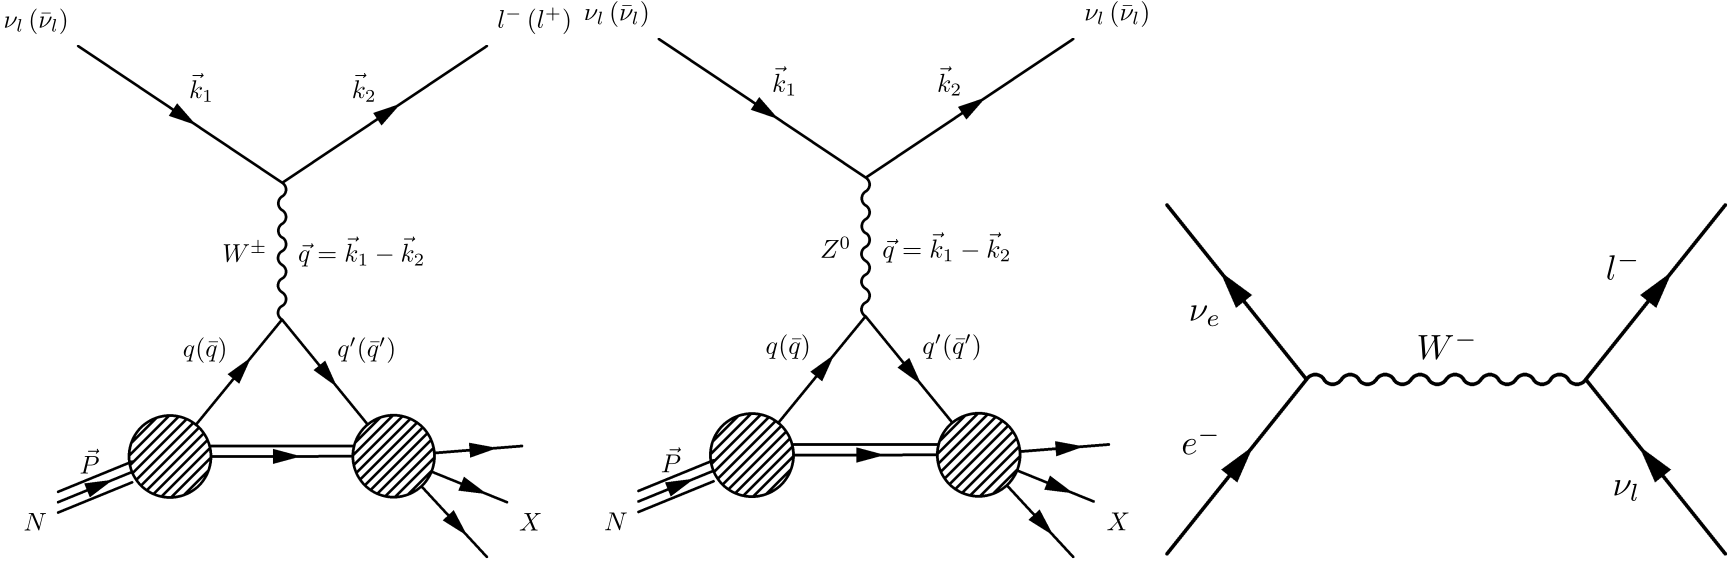
\includegraphics[width=\textwidth]{media/feynman_diagrams.png}

                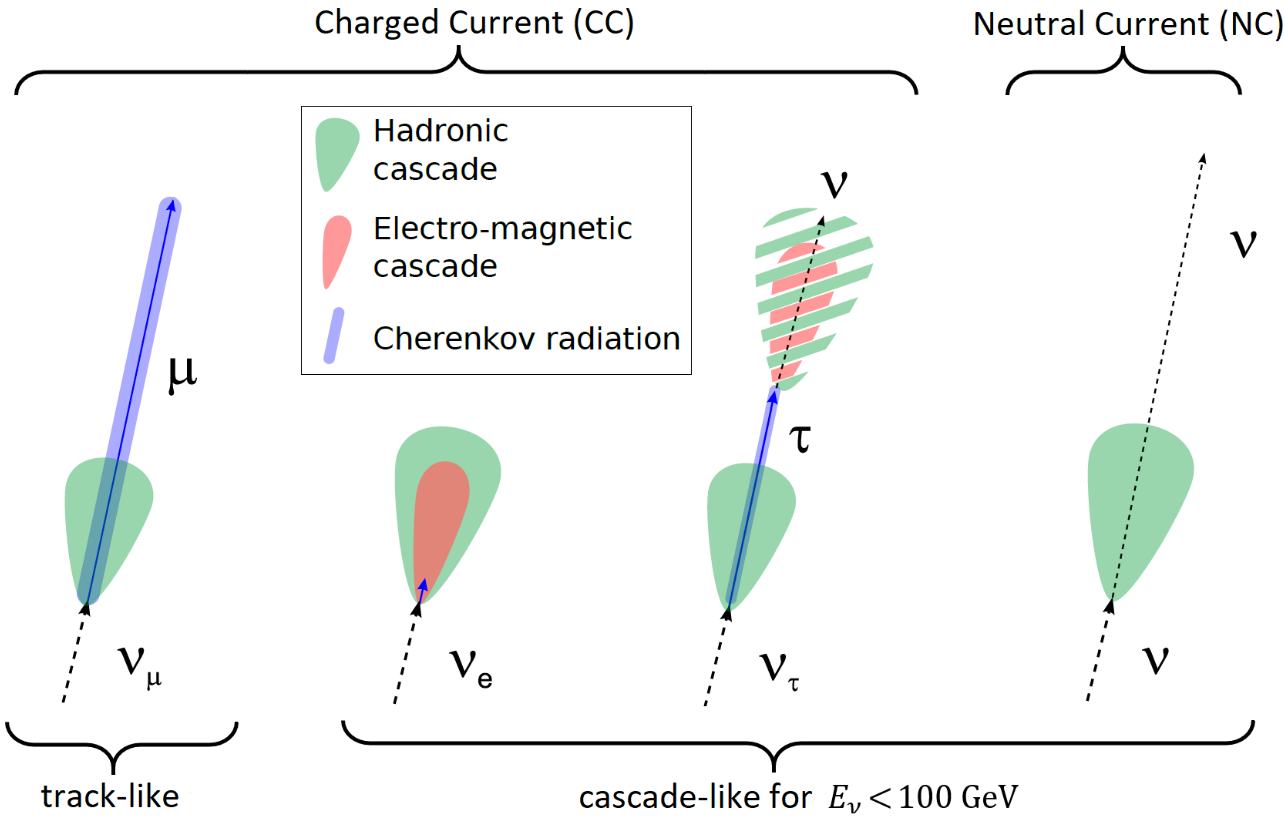
\includegraphics[width=.6\textwidth]{media/neutrino_interaction.png}
                \caption*{Feynman Diagrams and interaction signatures at Icecube \footnotemark[2]}
            \end{figure}
        \end{column}
    \end{columns}
    \footnotetext[1]{{\fullcite{aker2022direct}}}
    \footnotetext[2]{{\fullcite{reimann2020search}}}
\end{frame}
\begin{frame}{The Icecube Observatory\dots}
    \begin{columns}
        \hspace{-3em}
        \begin{column}{.6\textwidth}
            \vspace{-2em}
            \begin{figure}
                \centering
                \begin{tikzpicture}[tdplot_main_coords]
                    \node at (0, 0){
                        \def\svgwidth{1\textwidth}
                        \graphicspath{{media/}}
                        \fontsize{6}{4}\selectfont
                        \input{media/icecube_opt.pdf_tex}
                    };
                \end{tikzpicture}
                \vspace{-2em}
                \caption*{\small Modified from \fullcite{reimann2020search} }
            \end{figure}
        \end{column}
        \hspace{-2em}
        \begin{column}{.4\textwidth}
            \begin{itemize}
                \item[\textbf{\dots}] is located at the South-Pole.
                \item[\textbf{\dots}] finished construction in 2010.
                \item[\textbf{\dots}] has \SI{1}{\kilo\meter\tothe{3}} total volume.
                \item[\textbf{\dots}] can detect (InIce): $E_{\nu} = \mathcal{O}\l(\unit{\tera\electronvolt}\r)-\mathcal{O}\l(\unit{\peta\electronvolt}\r)$.
                \item[\textbf{\dots}] can detect (DeepCore): $E_{\nu} > \SI{10}{\giga\electronvolt}$.
            \end{itemize}
        \end{column}
        \hspace{2em}
    \end{columns}
\end{frame}

\begin{frame}{The Icecube Observatory Vocabulary}
    \begin{columns}
        \hspace{-3em}
        \begin{column}{.6\textwidth}
            \vspace{-2em}
            \begin{figure}
                \centering
                \begin{tikzpicture}[tdplot_main_coords]
                    \node at (0, 0){
                        \def\svgwidth{1\textwidth}
                        \graphicspath{{media/}}
                        \fontsize{6}{4}\selectfont
                        \input{media/icecube_opt.pdf_tex}
                    };
                    \coordinate (O) at (2,2.5,3.5);
                    \draw[thick,->] (O) -- +(2,0,0) node[anchor=north east, shift={(-.2,.1)}]{\small$x$};
                    \draw[thick,->] (O) -- +(0,2,0) node[anchor=west]{\small$y$};
                    \draw[thick,->] (O) -- +(0,0,2) node[anchor=east]{\small$z$};
                    \tdplotsetcoord{P}{\rvec}{\thetavec}{\phivec}
                    \draw[stealth-,color=mLightBrown] (O) -- +(P) node[above right] {$\nu$};
                    \draw[dashed, color=mLightBrown] (O) -- +(Pxy);
                    \draw[dashed, color=mLightBrown] (O)+(P) -- +(Pxy);
                    \tdplotdrawarc{(O)}{1}{0}{\phivec}{anchor=south, shift={(.2,-.1)}}{\small$\phi$}
                    \tdplotsetthetaplanecoords{\phivec}
                    \tdplotdrawarc[tdplot_rotated_coords]{(O)}{1}{0}%
                    {\thetavec}{anchor=north,shift={(0,-.1)}}{\small$\theta$}
                \end{tikzpicture}
                \vspace{-2em}
                \caption*{\small Modified from \fullcite{reimann2020search} }
            \end{figure}
        \end{column}
        \hspace{2em}
        \begin{column}{.4\textwidth}
            \begin{itemize}
                \item [\textbf{Zenith}] $\theta$
                \item [\textbf{Azimuth}] $\phi$
                      \pause
                \item [\textbf{DOM}] Digital-Optical-Module (PMT)
                \item [\textbf{InIce}] 78 strings\\ each 60 DOMs\\ DOM-to-DOM: \SI{17}{\meter}
                      string-to-string: \SI{125}{\meter}
                \item [\textbf{Deep Core}] 8 high efficiency strings
                      string-to-string: \SI{75}{\meter}
                      \pause
                \item [\textbf{$\hookrightarrow$Upper}]  10 DOMS, DOM-to-DOM: \SI{10}{\meter}
                \item [\textbf{$\hookrightarrow$Lower}]  50 DOMS, DOM-to-DOM: \SI{7}{\meter}
            \end{itemize}
        \end{column}
        \hspace{-2em}
    \end{columns}
\end{frame}
\begin{frame}{Methods of Reconstruction}
    \centering
    \begin{columns}[T]
        \begin{column}{.25\textwidth}
            LineFit\\
            \begin{equation*}
                \min_{\vec{x}_0, \vec v} \sum_{i=1}^{N}\abs{\vec x_i - \l(\vec{x}_{0}+\vec v t_i\r)}^2
            \end{equation*}
            \begin{itemize}
                \item Minimize square error
                \item Simple first guess
                \item Not much physics \enquote{input}
            \end{itemize}
        \end{column}
        \pause
        \begin{column}{.35\textwidth}
            MPEFit\\
            \begin{equation*}
                \max_{\vec{r}_0, t_0, \phi, \theta} \prod_{i=1}^{N} p\l(t_{i,\mathrm{res}}\middle|\vec{r}_0, t_0, \vec d(\phi, \theta)\r)
            \end{equation*}
            \begin{itemize}
                \item Maximize Likelihood $\mathcal L$
                \item Complex
                \item A lot of physics input
                \item Uncertainty by varying $\mathcal L$(Paraboloid)
            \end{itemize}
        \end{column}
        \pause
        \begin{column}{.4\textwidth}
            Machine Learning \\
            \begin{equation*}
                \min_{\vec p} \frac{1}{N}\sum_{i=1}^{N} L(y_{\mathrm{pred}}=\hat{f}\l(\mathbf{X_i} \middle | \vec p\r), y_{i,\mathrm{true}})
            \end{equation*}

            \begin{itemize}
                \item Minimize empirical loss-function $\mathbf L$
                \item Training the $\vec p$ is complex, but applying is simple
                \item No physics input, except true label $y_{i,\mathrm{true}}$
                \item Uncertainty from estimator $\hat f$
            \end{itemize}
        \end{column}
    \end{columns}
\end{frame}
\begin{frame}{Monte Carlo Simulation}
    From where do we get the true labels, e.g $E, \theta$ or $\phi$?
    $\rightarrow$ \textbf{Monte Carlo Simulation} \\
    \vspace{1em}
    \begin{center}
        Generate Primary Particle ($E_\nu, \theta, \phi$)\\
        $\downarrow$\\
        Propagation/Interaction/Decay
        \\$\downarrow$\\
            Detector interaction and response (DOM pulses)
            \\$\downarrow$\\
        Machine Learning input (e.g. $n$ features per DOM)
    \end{center}
    \pause
    \textbf{Do we trust our simulation data?}
\end{frame}
\section{DNN Software}

\section{What I Have Done}
\begin{frame}{General Remarks}
    \begin{itemize}
        \item \texttt{dnn\_reco} running on the IceCube servers and cluster @Wisconsin
        \item I modified a few python scripts of the original software to add minor functionalities\footnote{Can be found \href{https://github.com/The-Ludwig/dnn_reco}{here: github.com/The-Ludwig/dnn\_reco} }
        \item Submit-scripts to work with the cluster GPUs were created
        \item Noted where \texttt{dnn\_reco}'s documentation\footnote{Documentation can be found \href{https://user-web.icecube.wisc.edu/~mhuennefeld/docs/dnn_reco/html/pages/about.html}{here}} is out-of-date
    \end{itemize}

    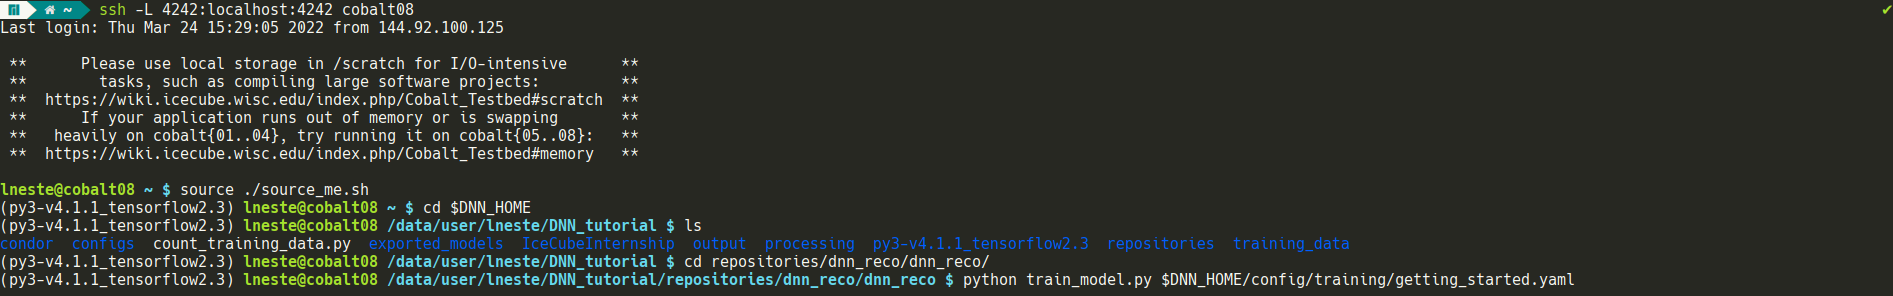
\includegraphics[width=\textwidth]{media/console.png}
\end{frame}
\begin{frame}{A First Model @13000 Training Iterations}
    \begin{columns}
        \begin{column}{.35\textwidth}
            \begin{tabular}{>{\small\bf}r l}
                \toprule
                Features                  & 9                \\
                Training Dataset          & L2 11883         \\
                Batch Size                & 32               \\
                UDC conv. layers          & 4                \\
                LDC conv. layers          & 8                \\
                Hex. conv. layers         & 8                \\
                Dense layers              & 1\times50        \\
                $\rightarrow$ Free Params & 24532            \\
                \midrule
                Test Dataset              & L2 11069         \\
                Loss function             & GL               \\
                Optimizer                 & ADAM             \\
                Learning Rate             & $10^{-3}$        \\
                Input Dropout Rate        & \SI{5}{\percent} \\
                \bottomrule
            \end{tabular}
        \end{column}
        \begin{column}{.65\textwidth}
            \begin{figure}
                \centering
                \only<1>{
                    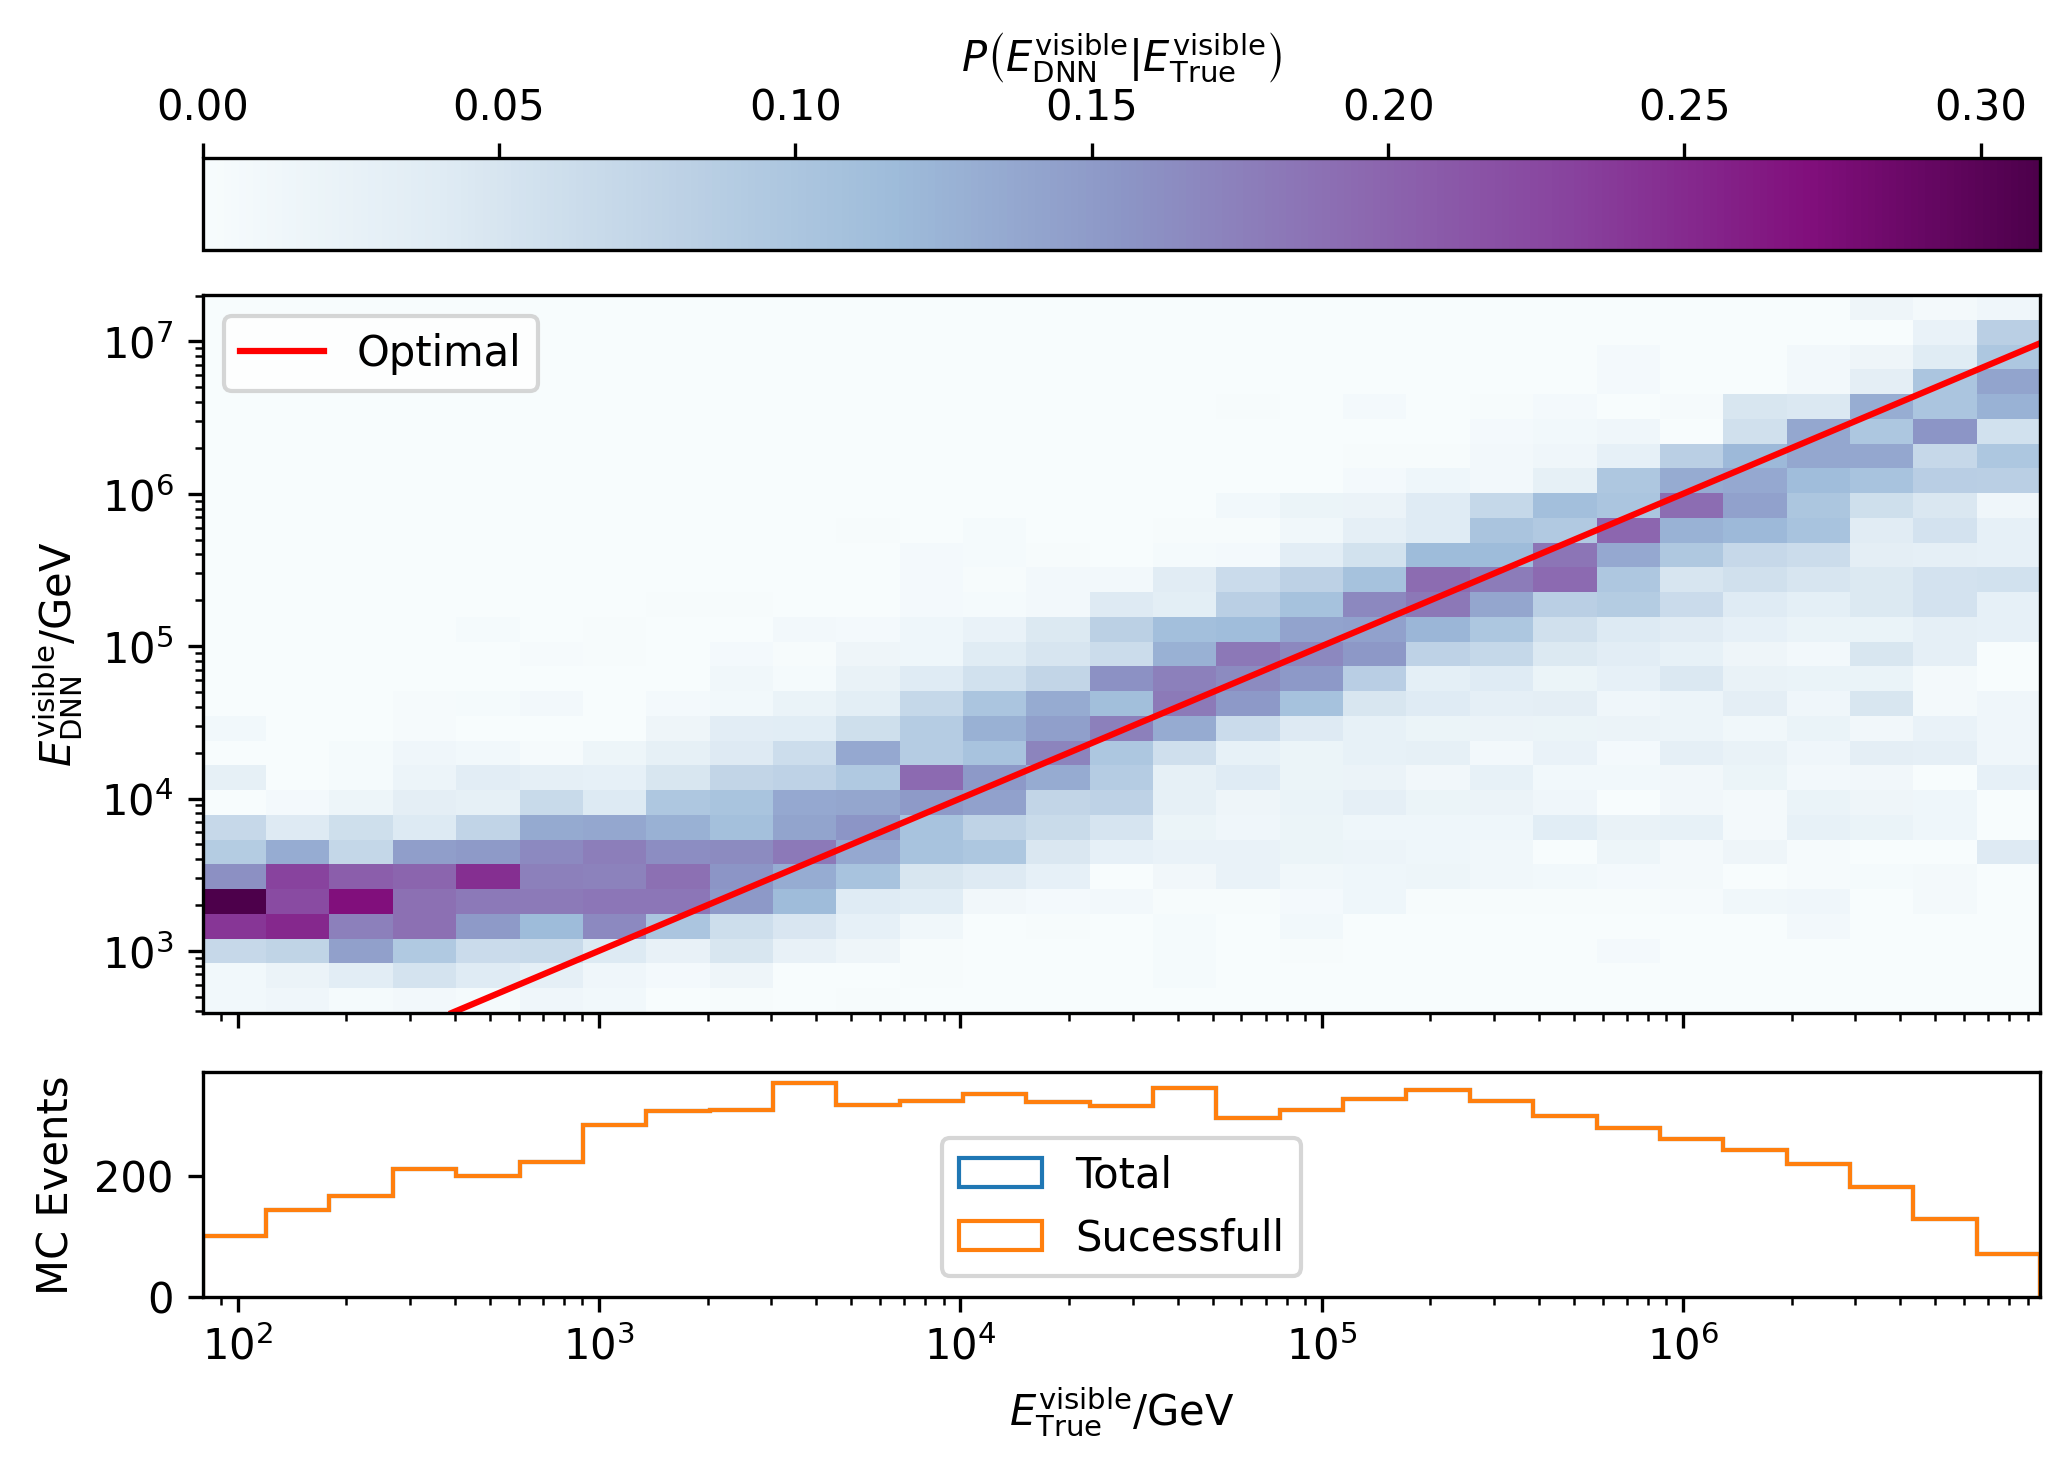
\includegraphics[width=.95\textwidth]{media/DNN_CORR.png}
                    \caption*{\small Normalized correlation plot of visible energy}
                }
                \only<2>{
                    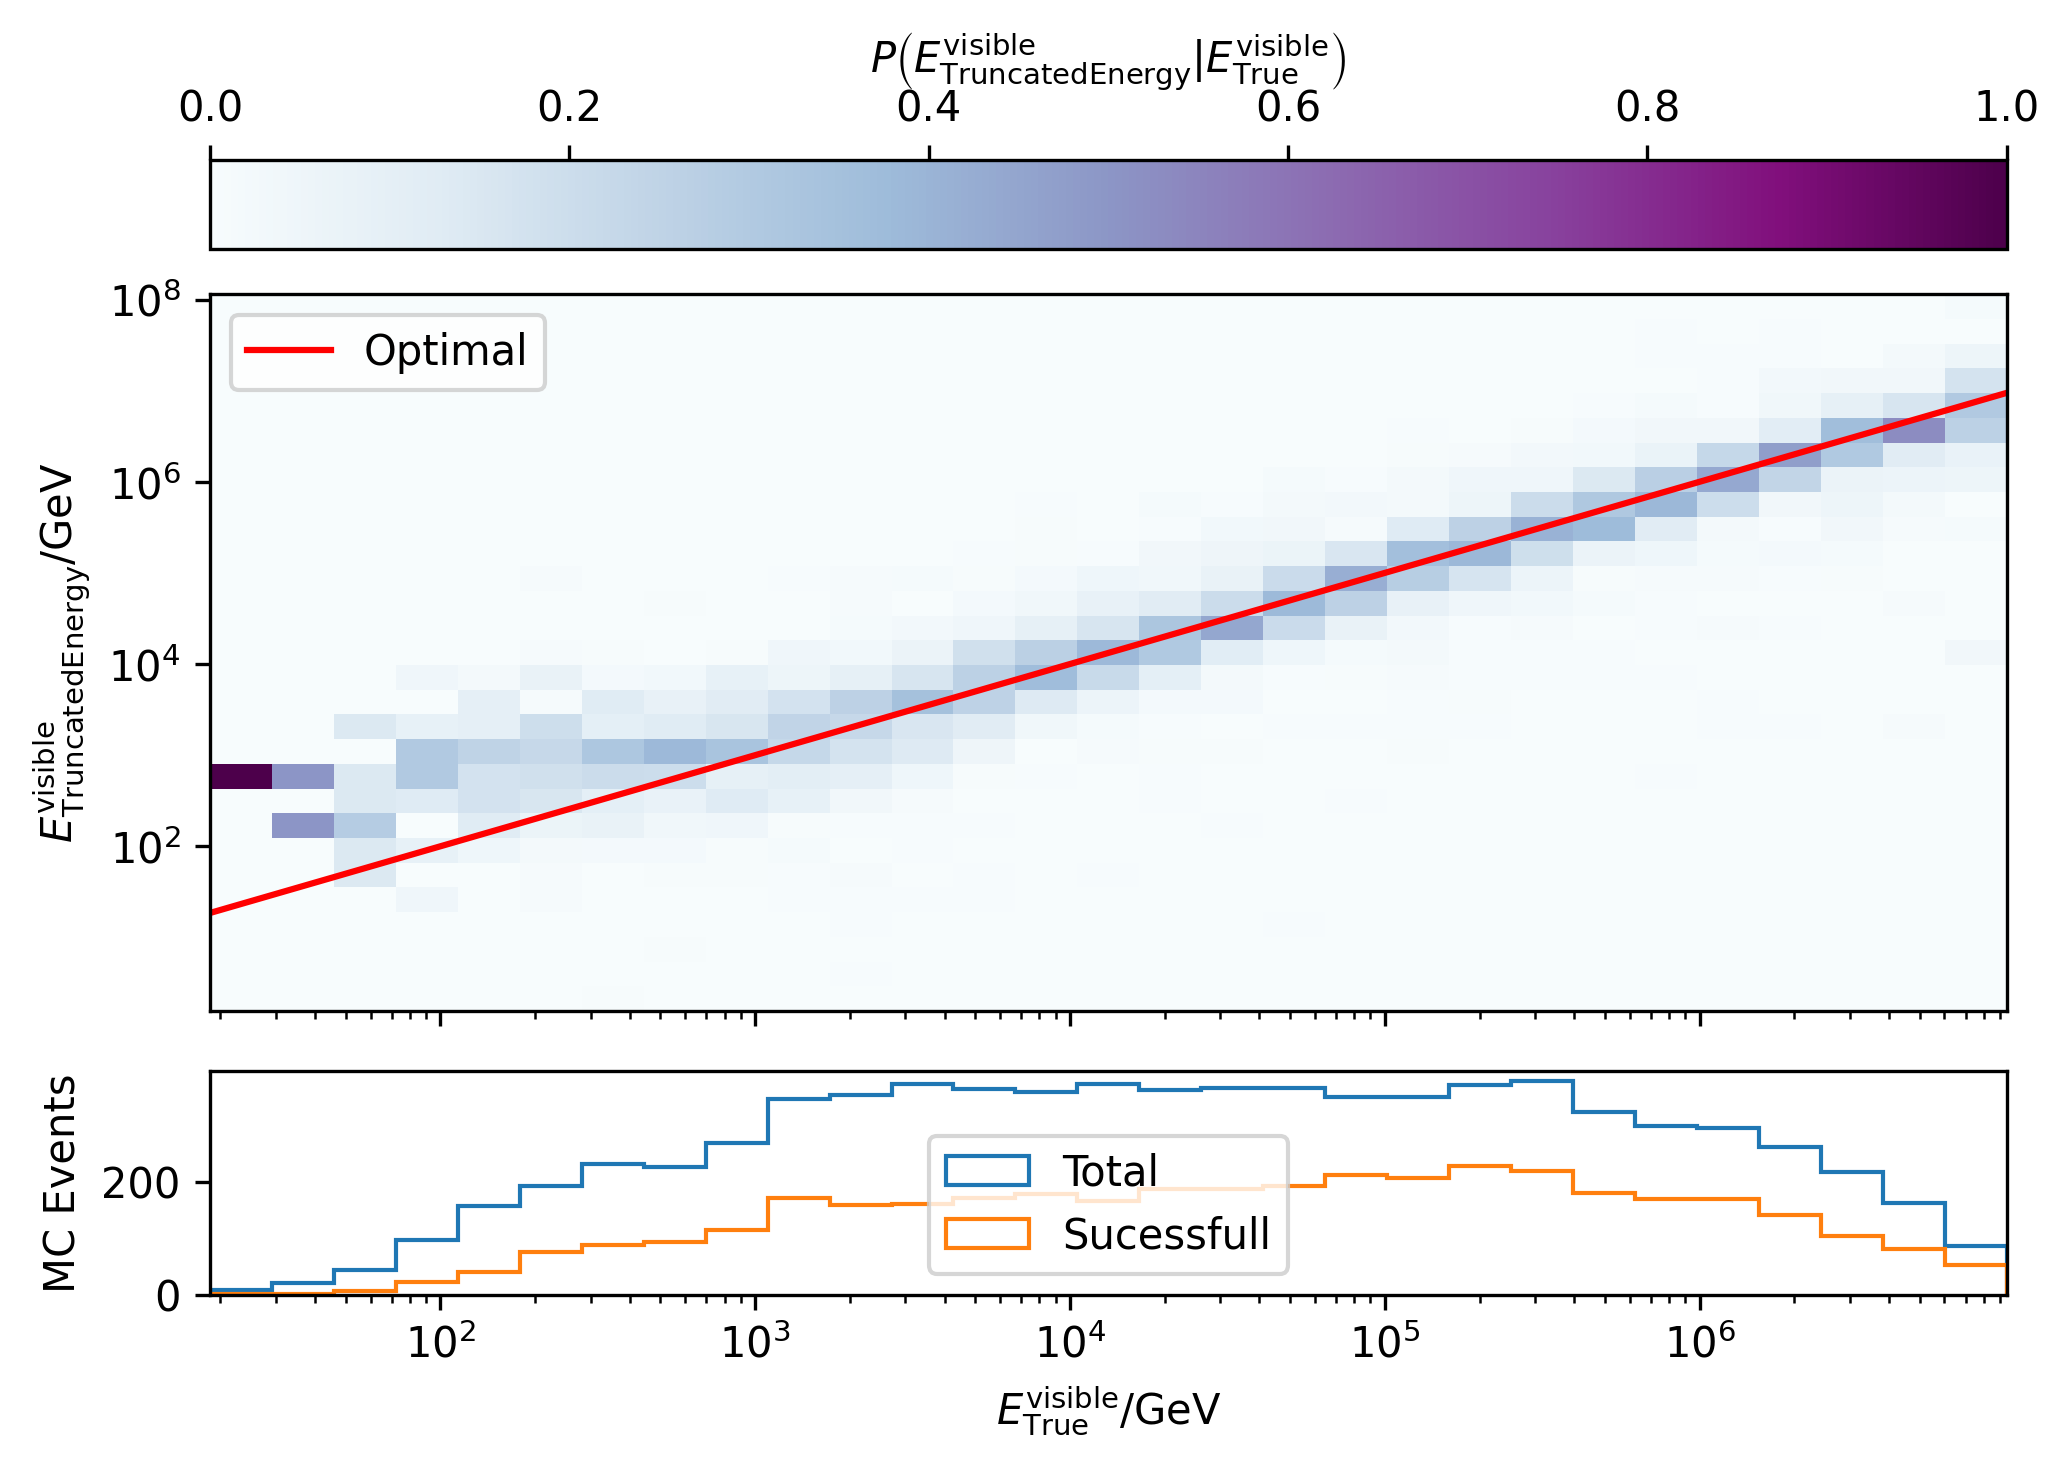
\includegraphics[width=.95\textwidth]{media/TRUN_CORR.png}
                    \caption*{\small Normalized correlation plot of visible energy (classical method)}
                }
            \end{figure}
        \end{column}
    \end{columns}
\end{frame}
\begin{frame}{A First Model for Directional Reconstruction}
    \begin{columns}
        \begin{column}{.35\textwidth}
            \begin{tabular}{>{\small\bf}r l}
                \toprule
                Features                  & 9         \\
                Training Dataset          & L2 11883  \\
                Batch Size                & 32        \\
                UDC conv. layers          & 4         \\
                LDC conv. layers          & 8         \\
                Hex. conv. layers         & 8         \\
                Dense layers              & 1\times50 \\
                $\rightarrow$ Free Params & 24532     \\
                \bottomrule
            \end{tabular}
        \end{column}
        \begin{column}{.65\textwidth}
            \begin{figure}
                \centering
                \only<1>{
                    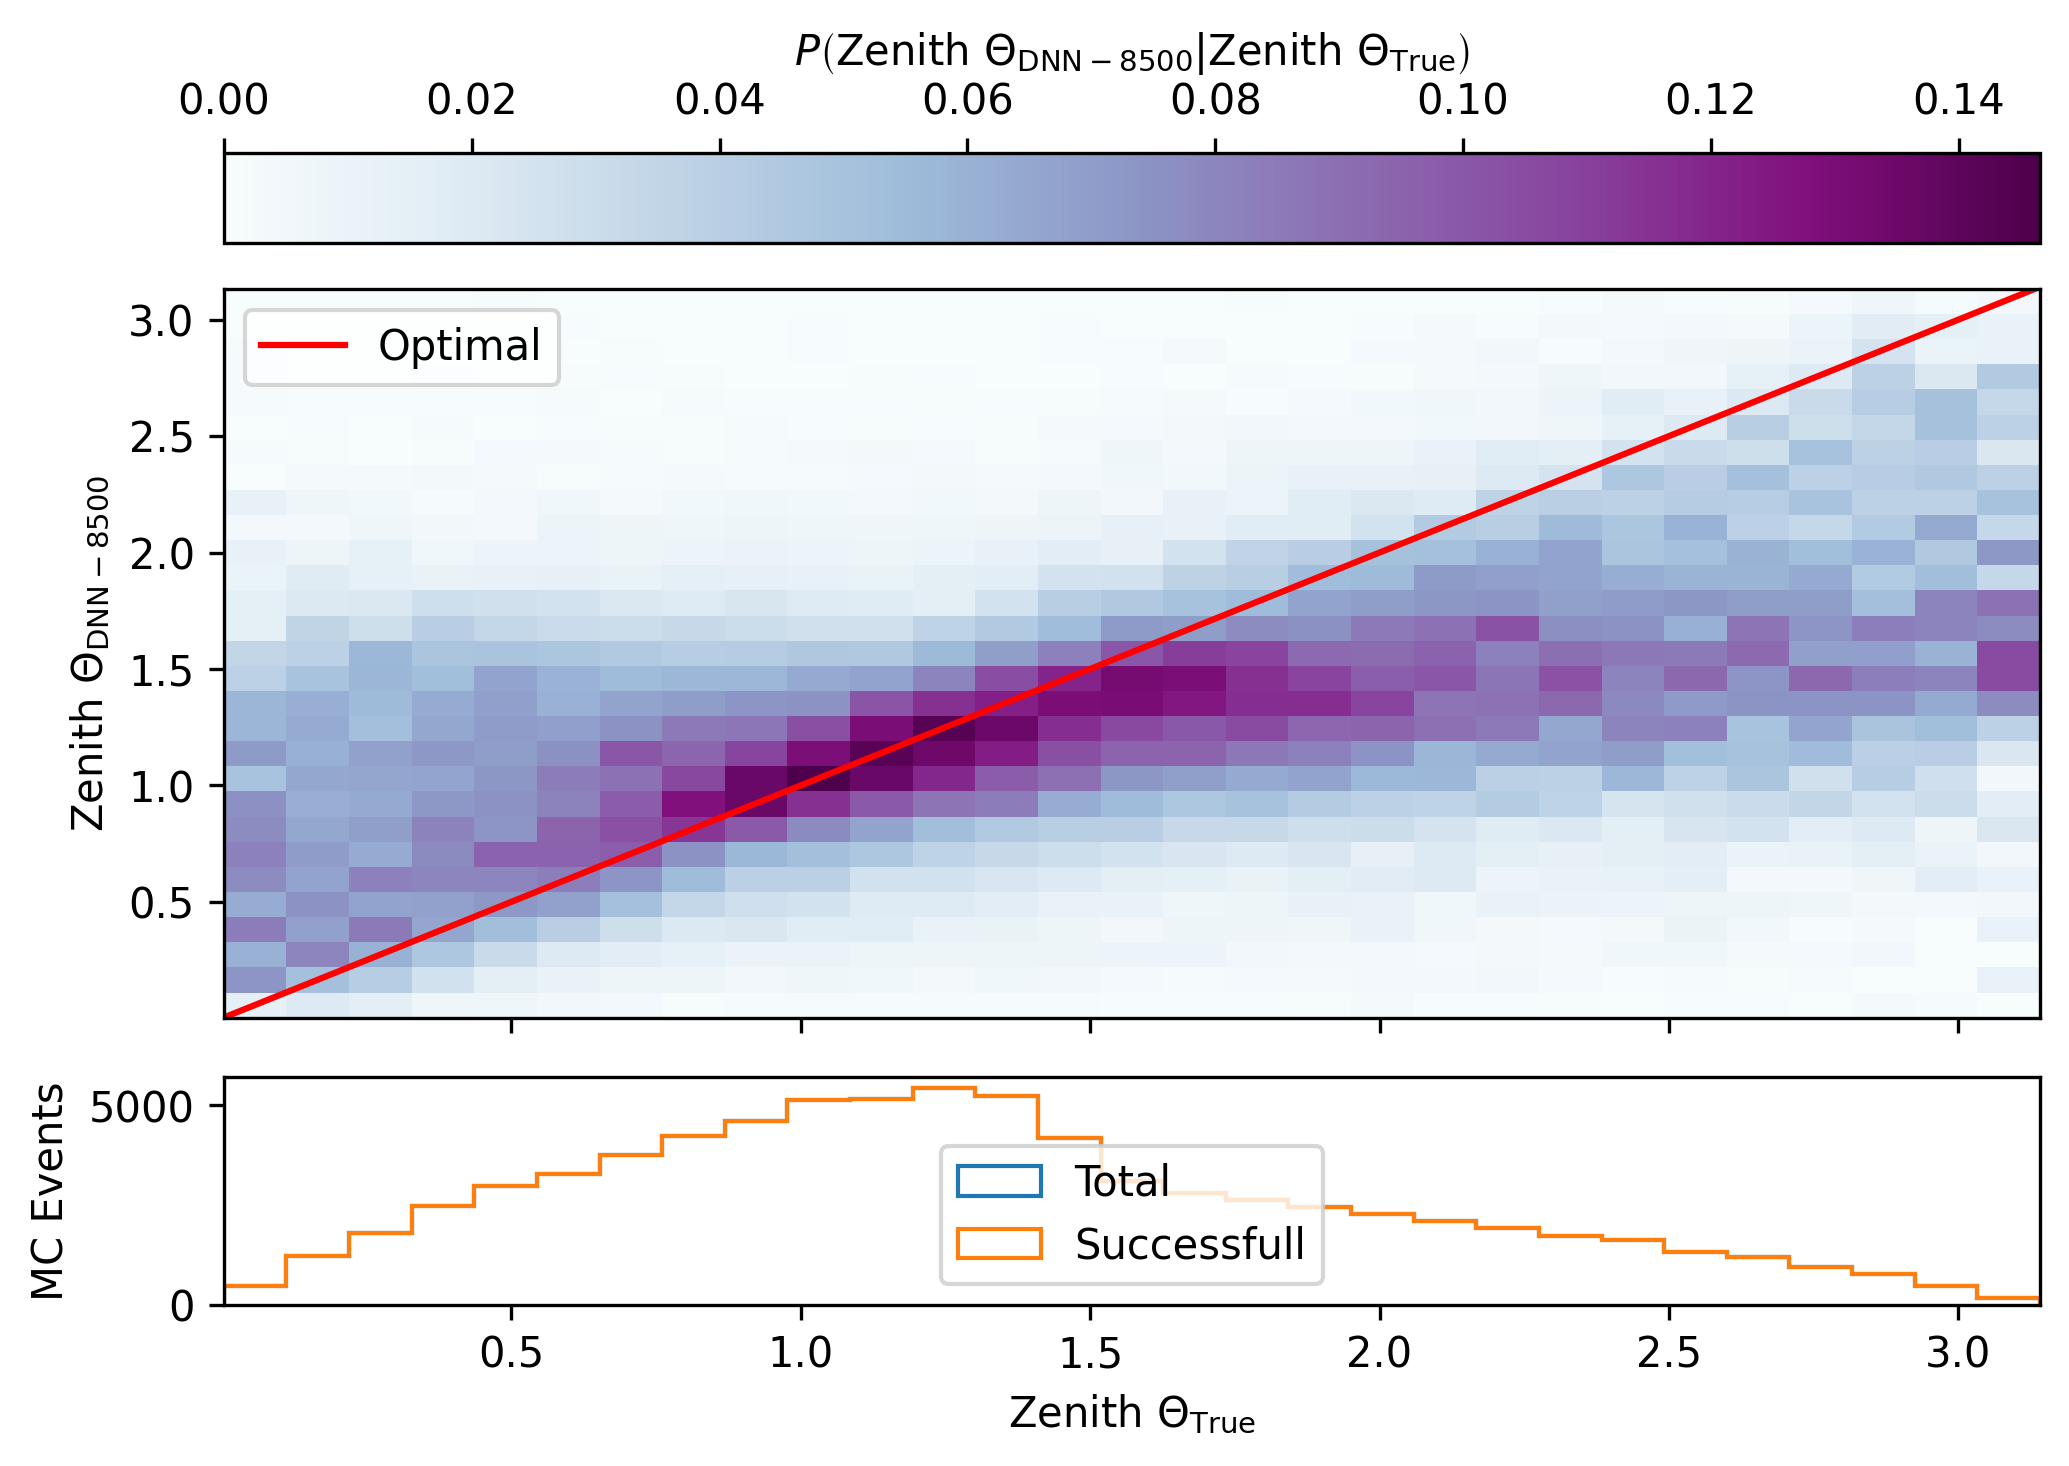
\includegraphics[width=.95\textwidth]{media/zenith_8500.png}
                    \caption*{\small Normalized zenith correlation @8500 training steps}
                }
                \only<2>{
                    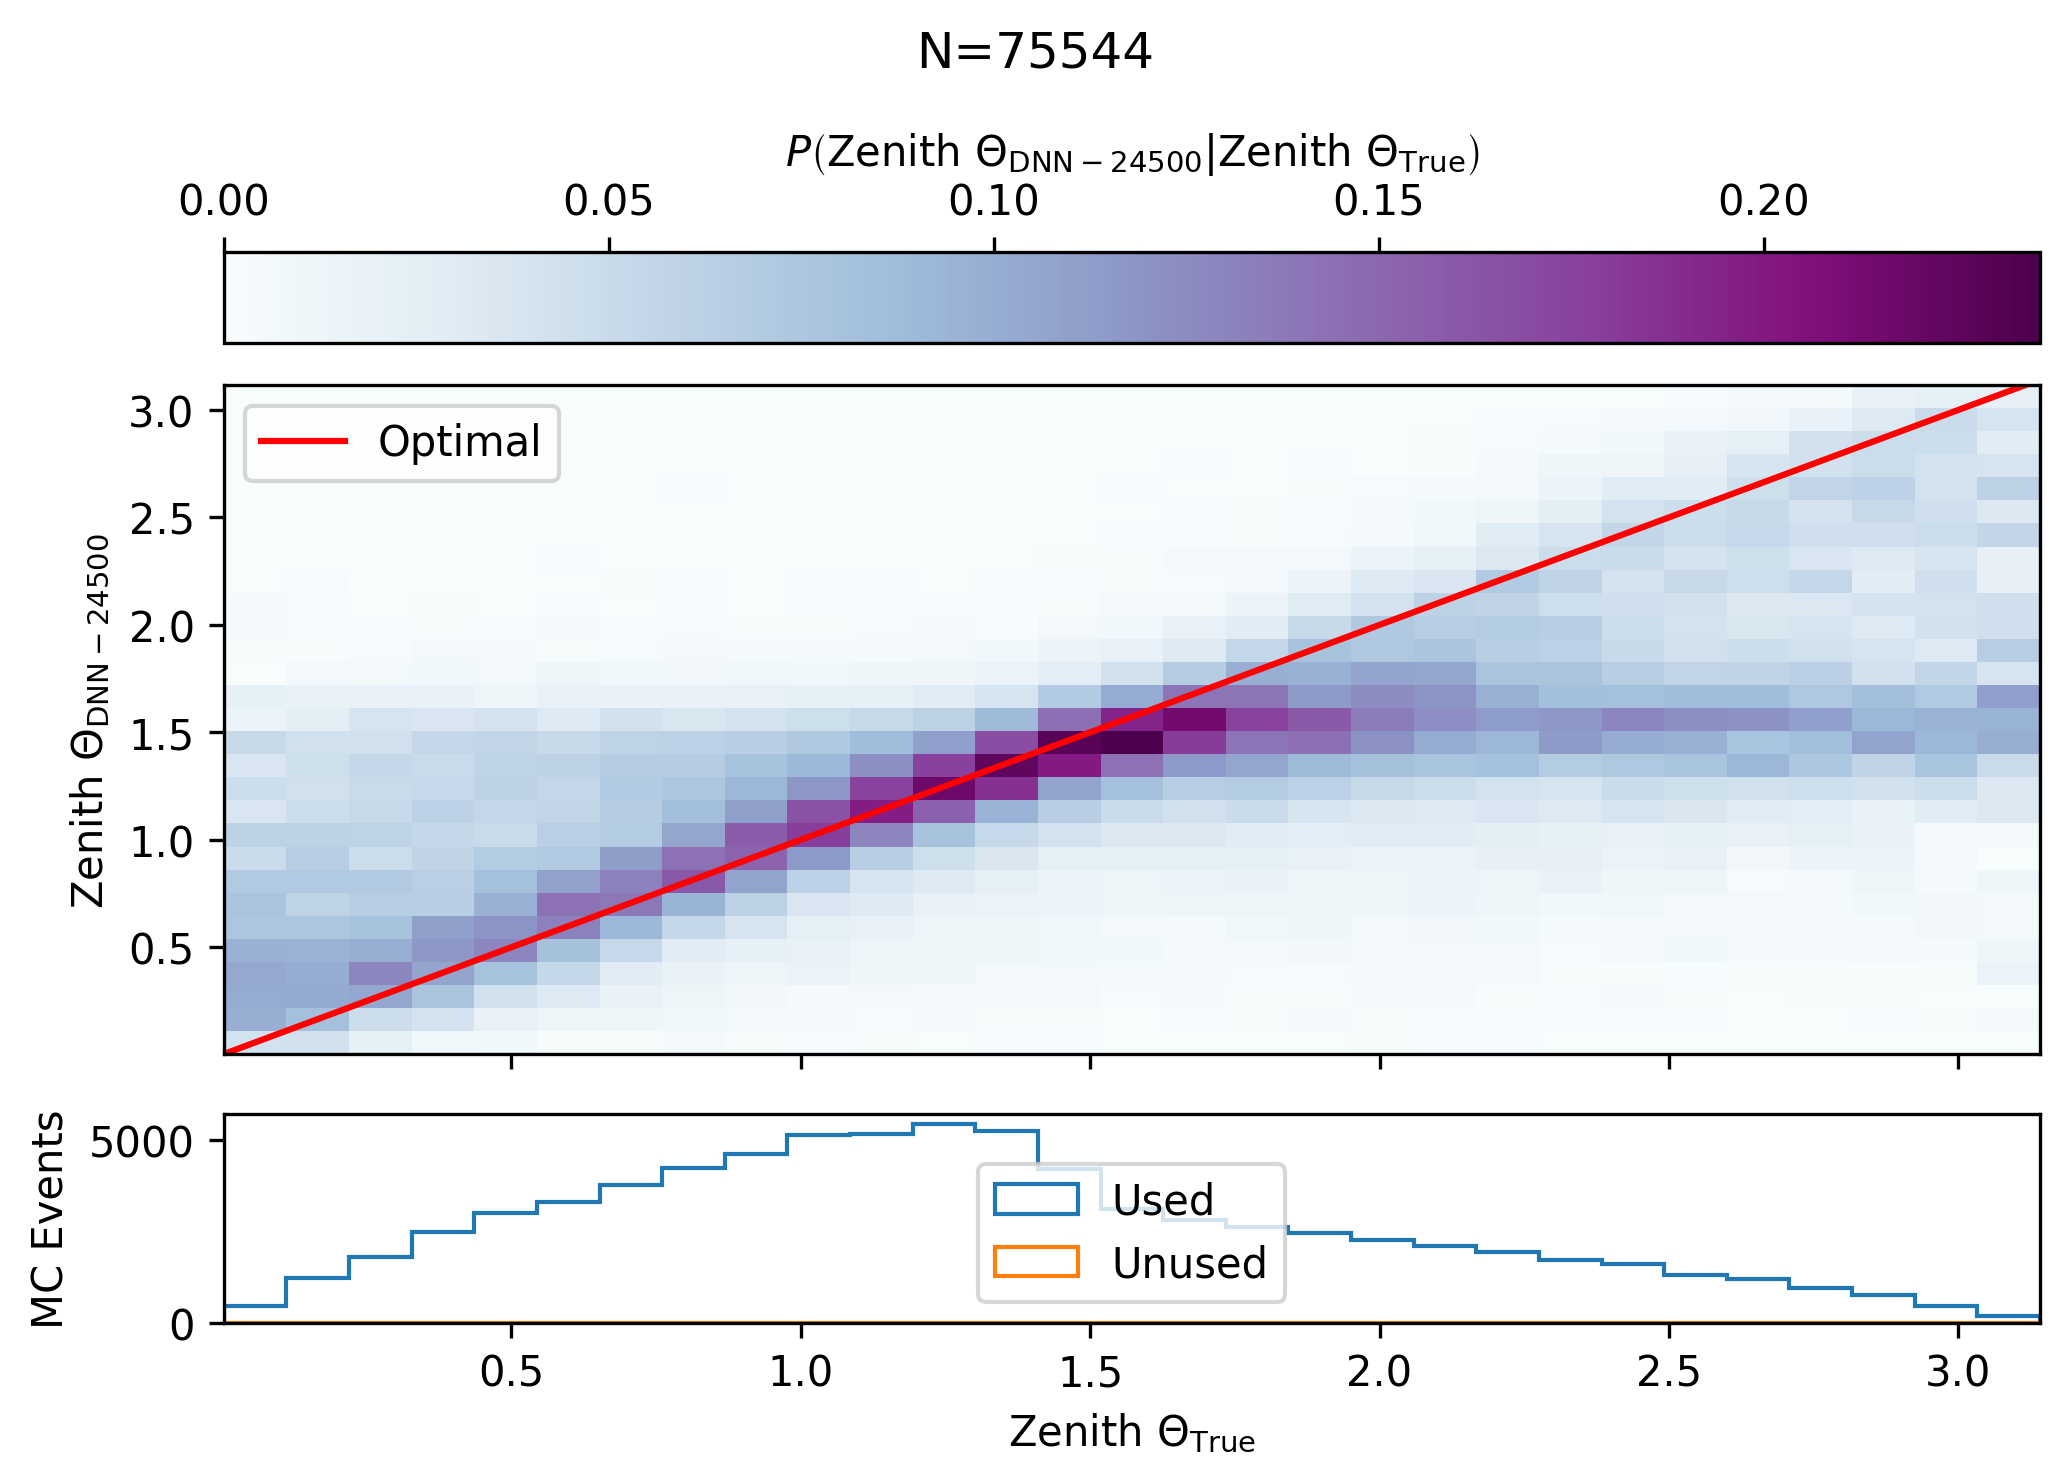
\includegraphics[width=.95\textwidth]{media/zenith_24500.png}
                    \caption*{\small Normalized zenith correlation @24500 training steps}
                }
                \only<3>{
                    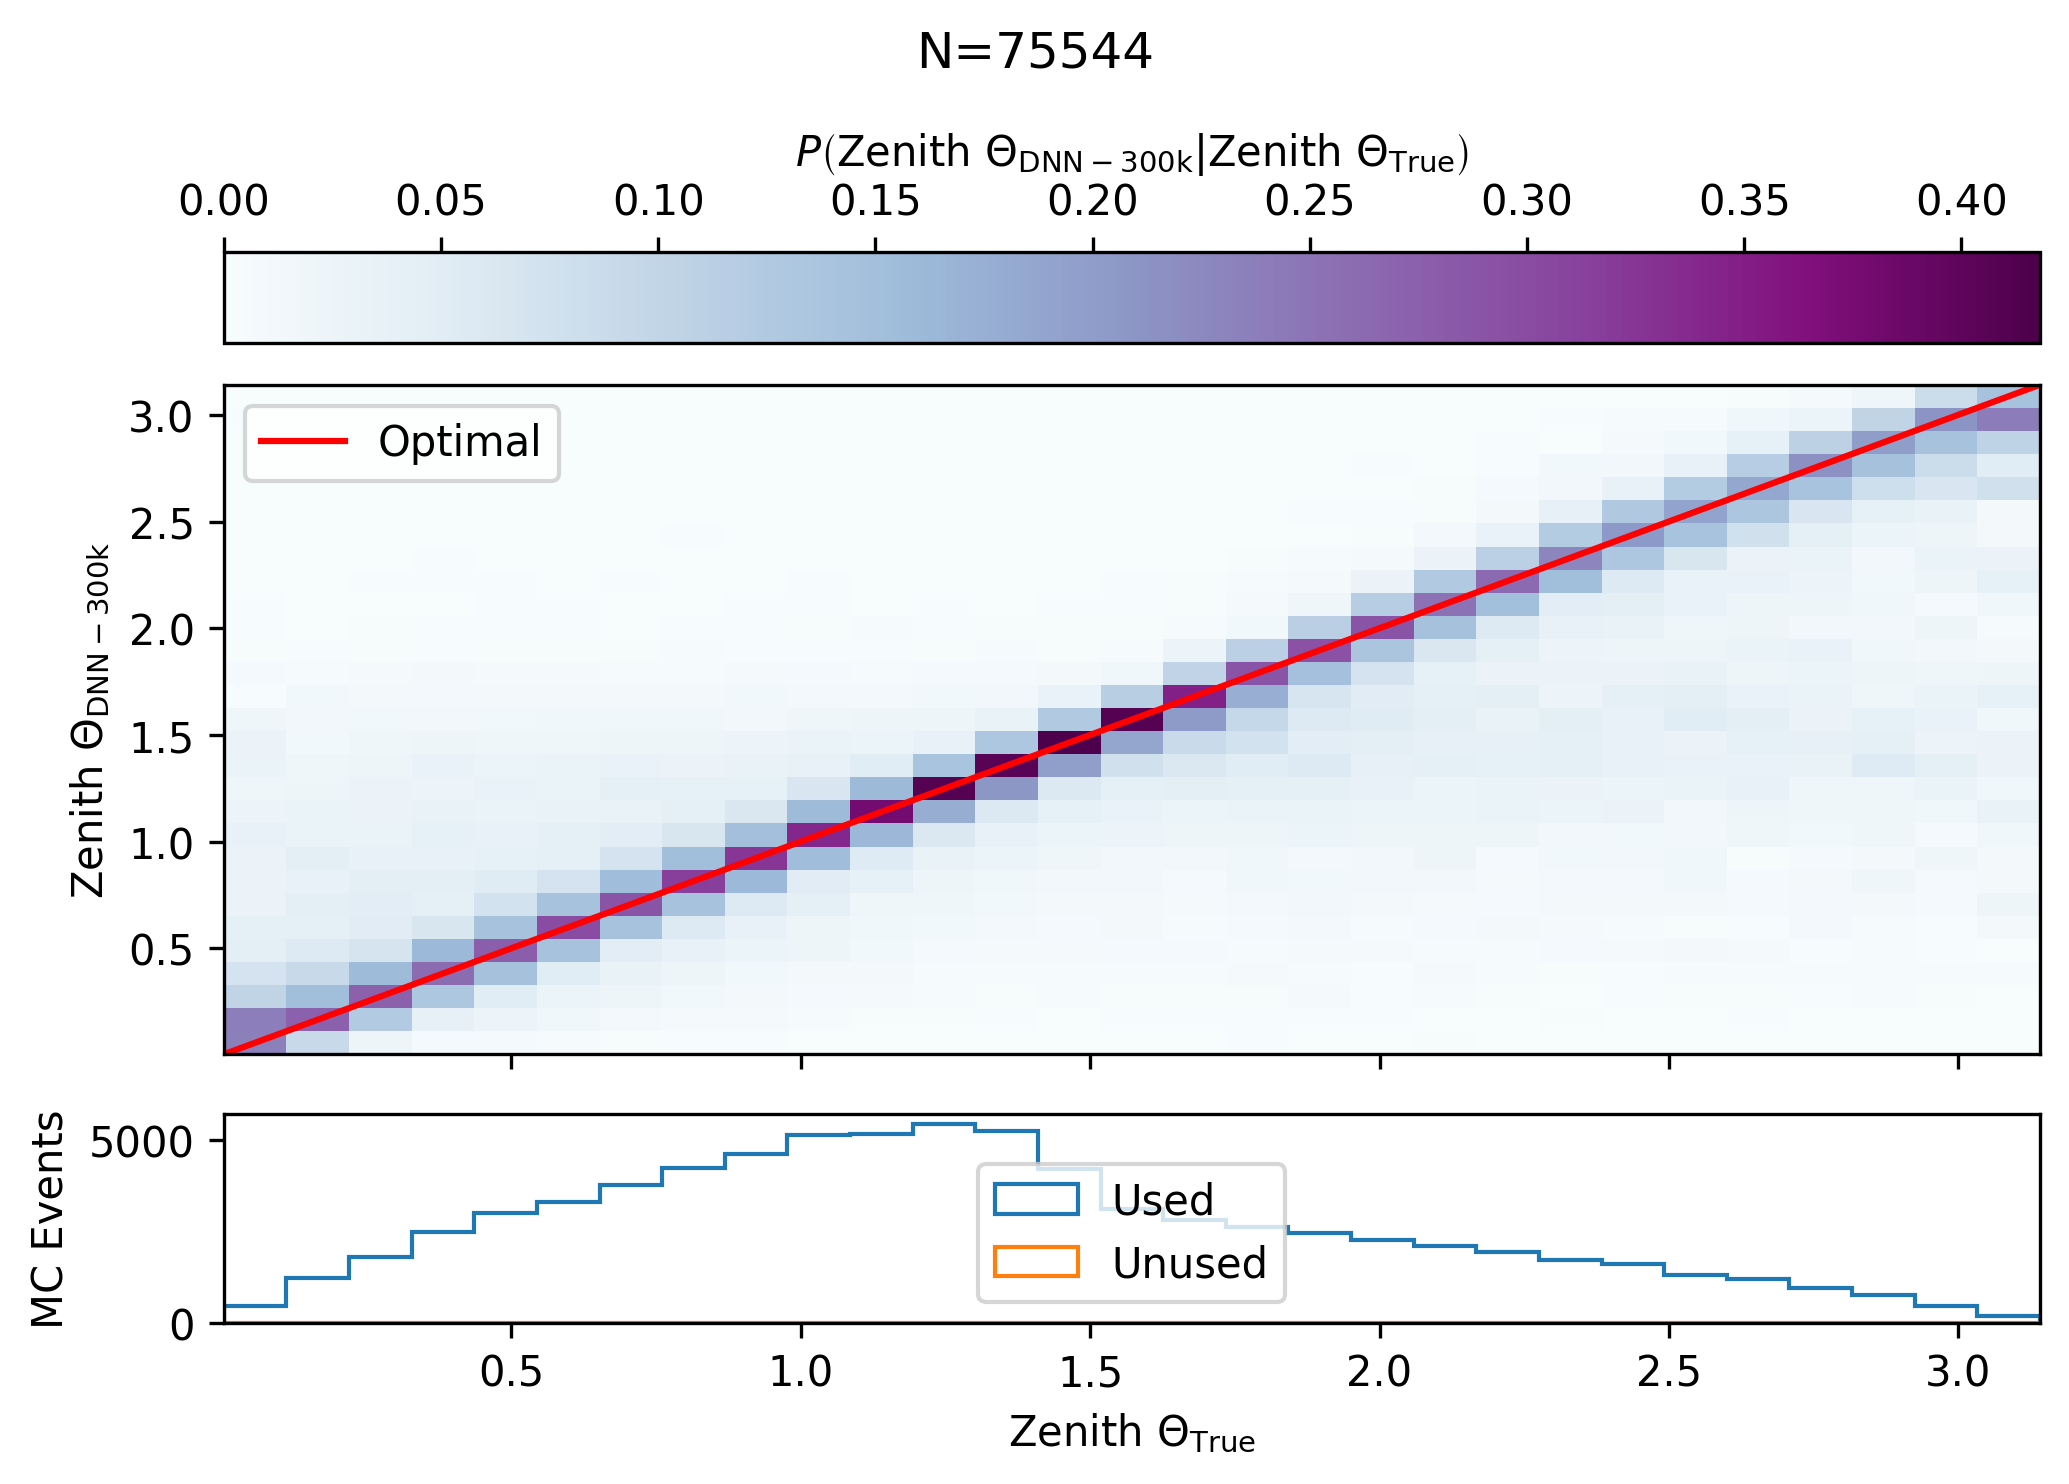
\includegraphics[width=.95\textwidth]{media/zenith_300k.png}
                    \caption*{\small Normalized zenith correlation @300k training steps}
                }
                \only<4>{
                    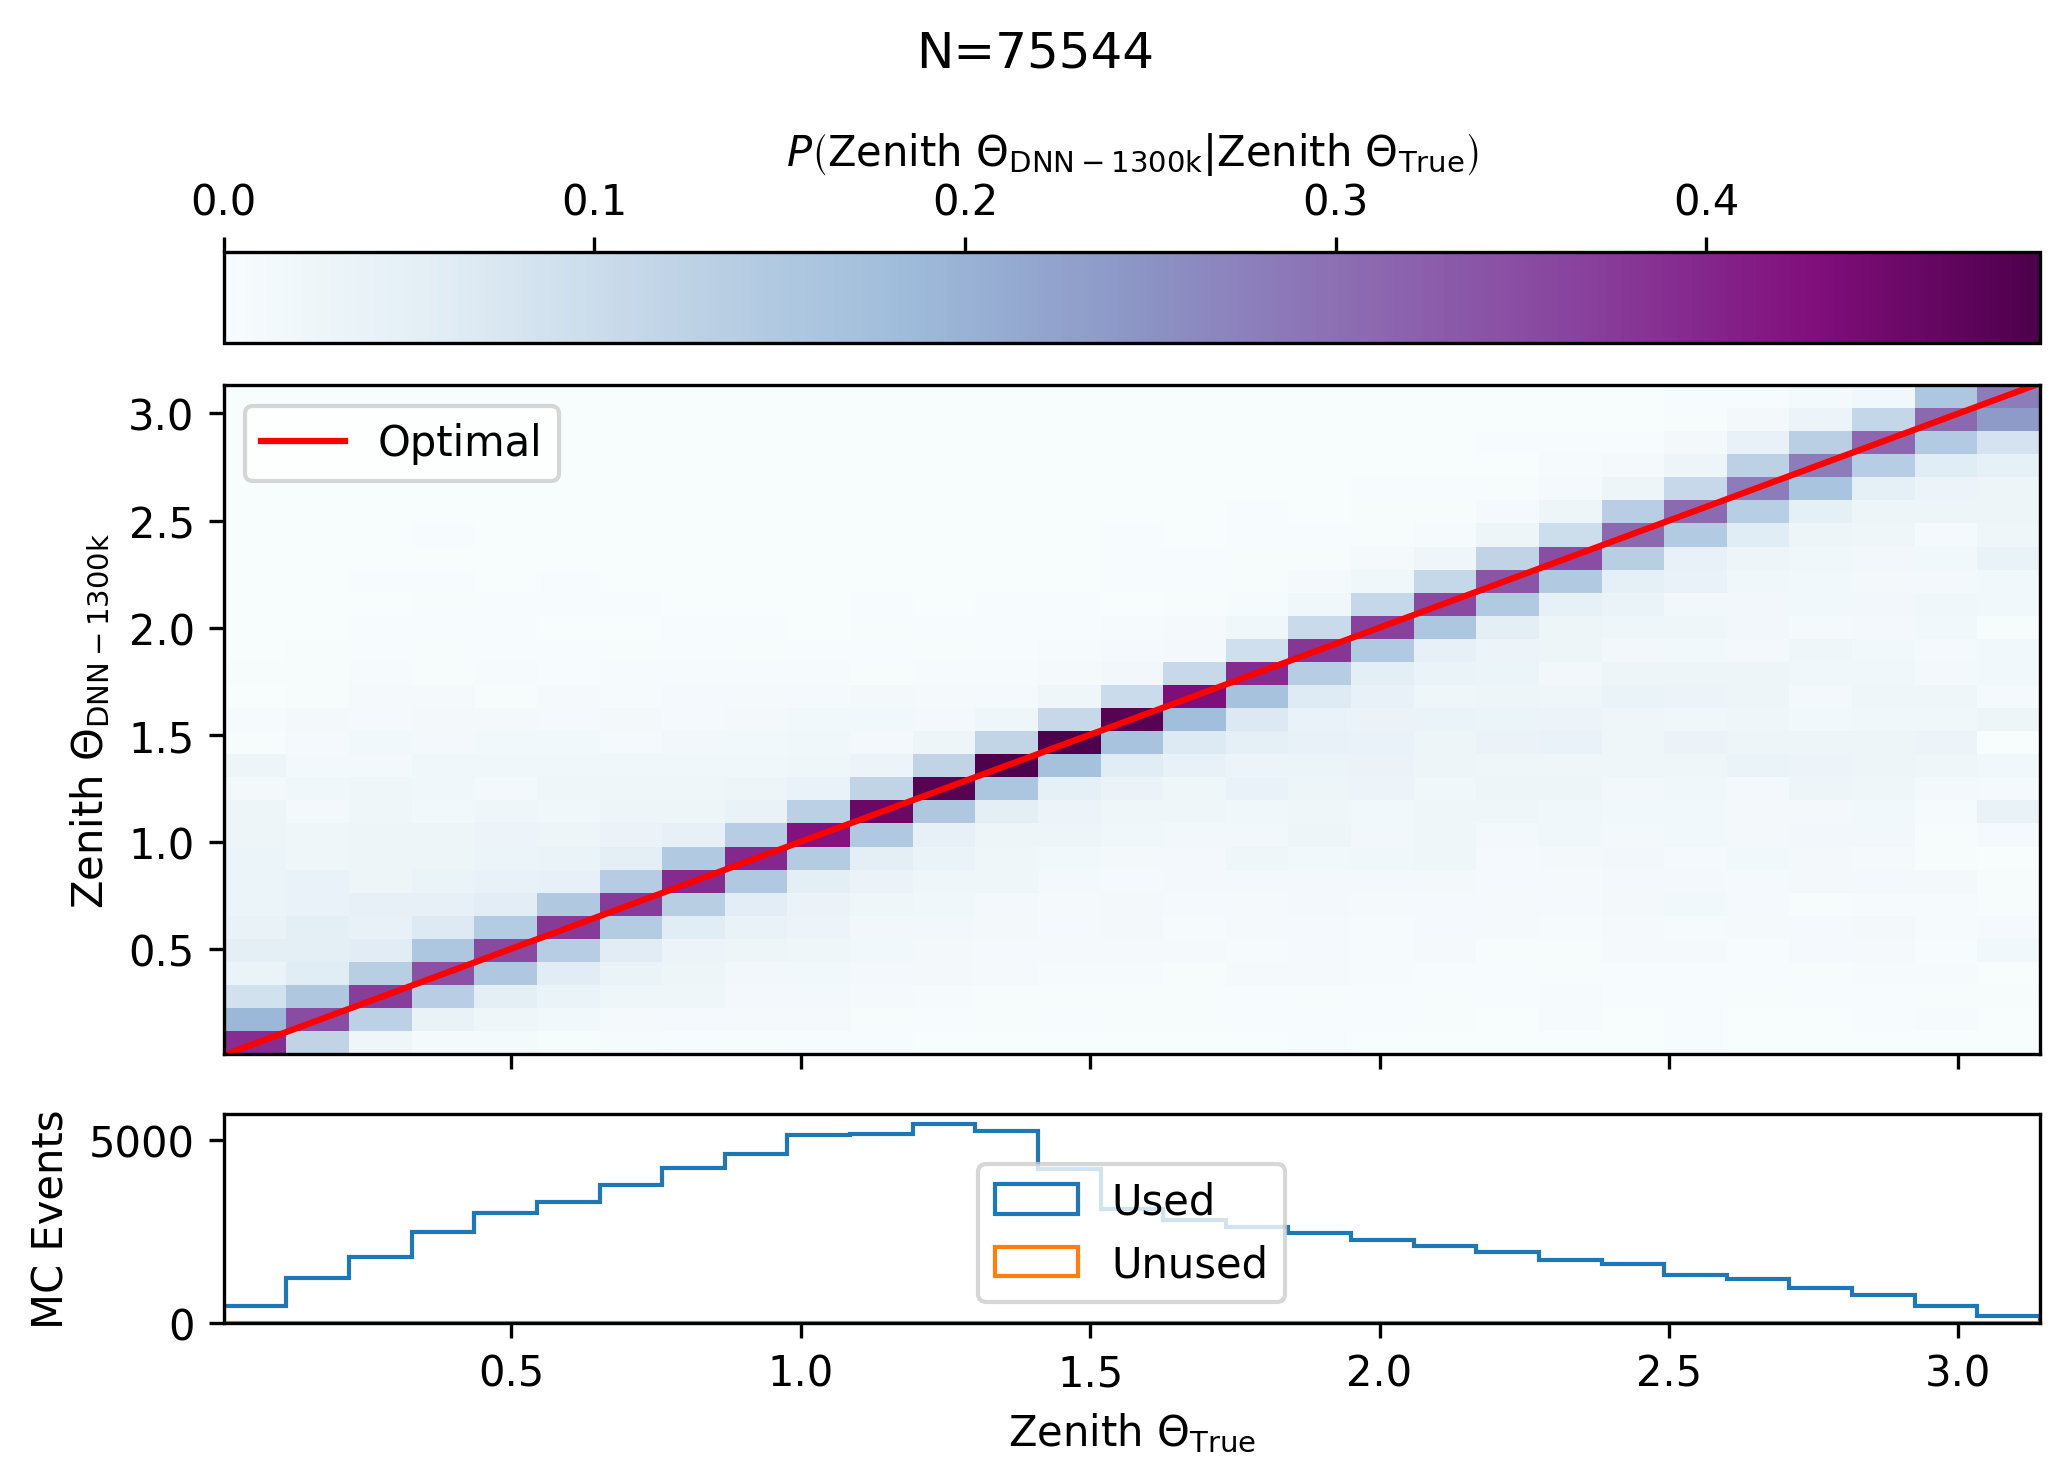
\includegraphics[width=.95\textwidth]{media/zenith_1.5m.png}
                    \caption*{\small Normalized zenith correlation @1.3m training steps}
                }
                \only<5>{
                    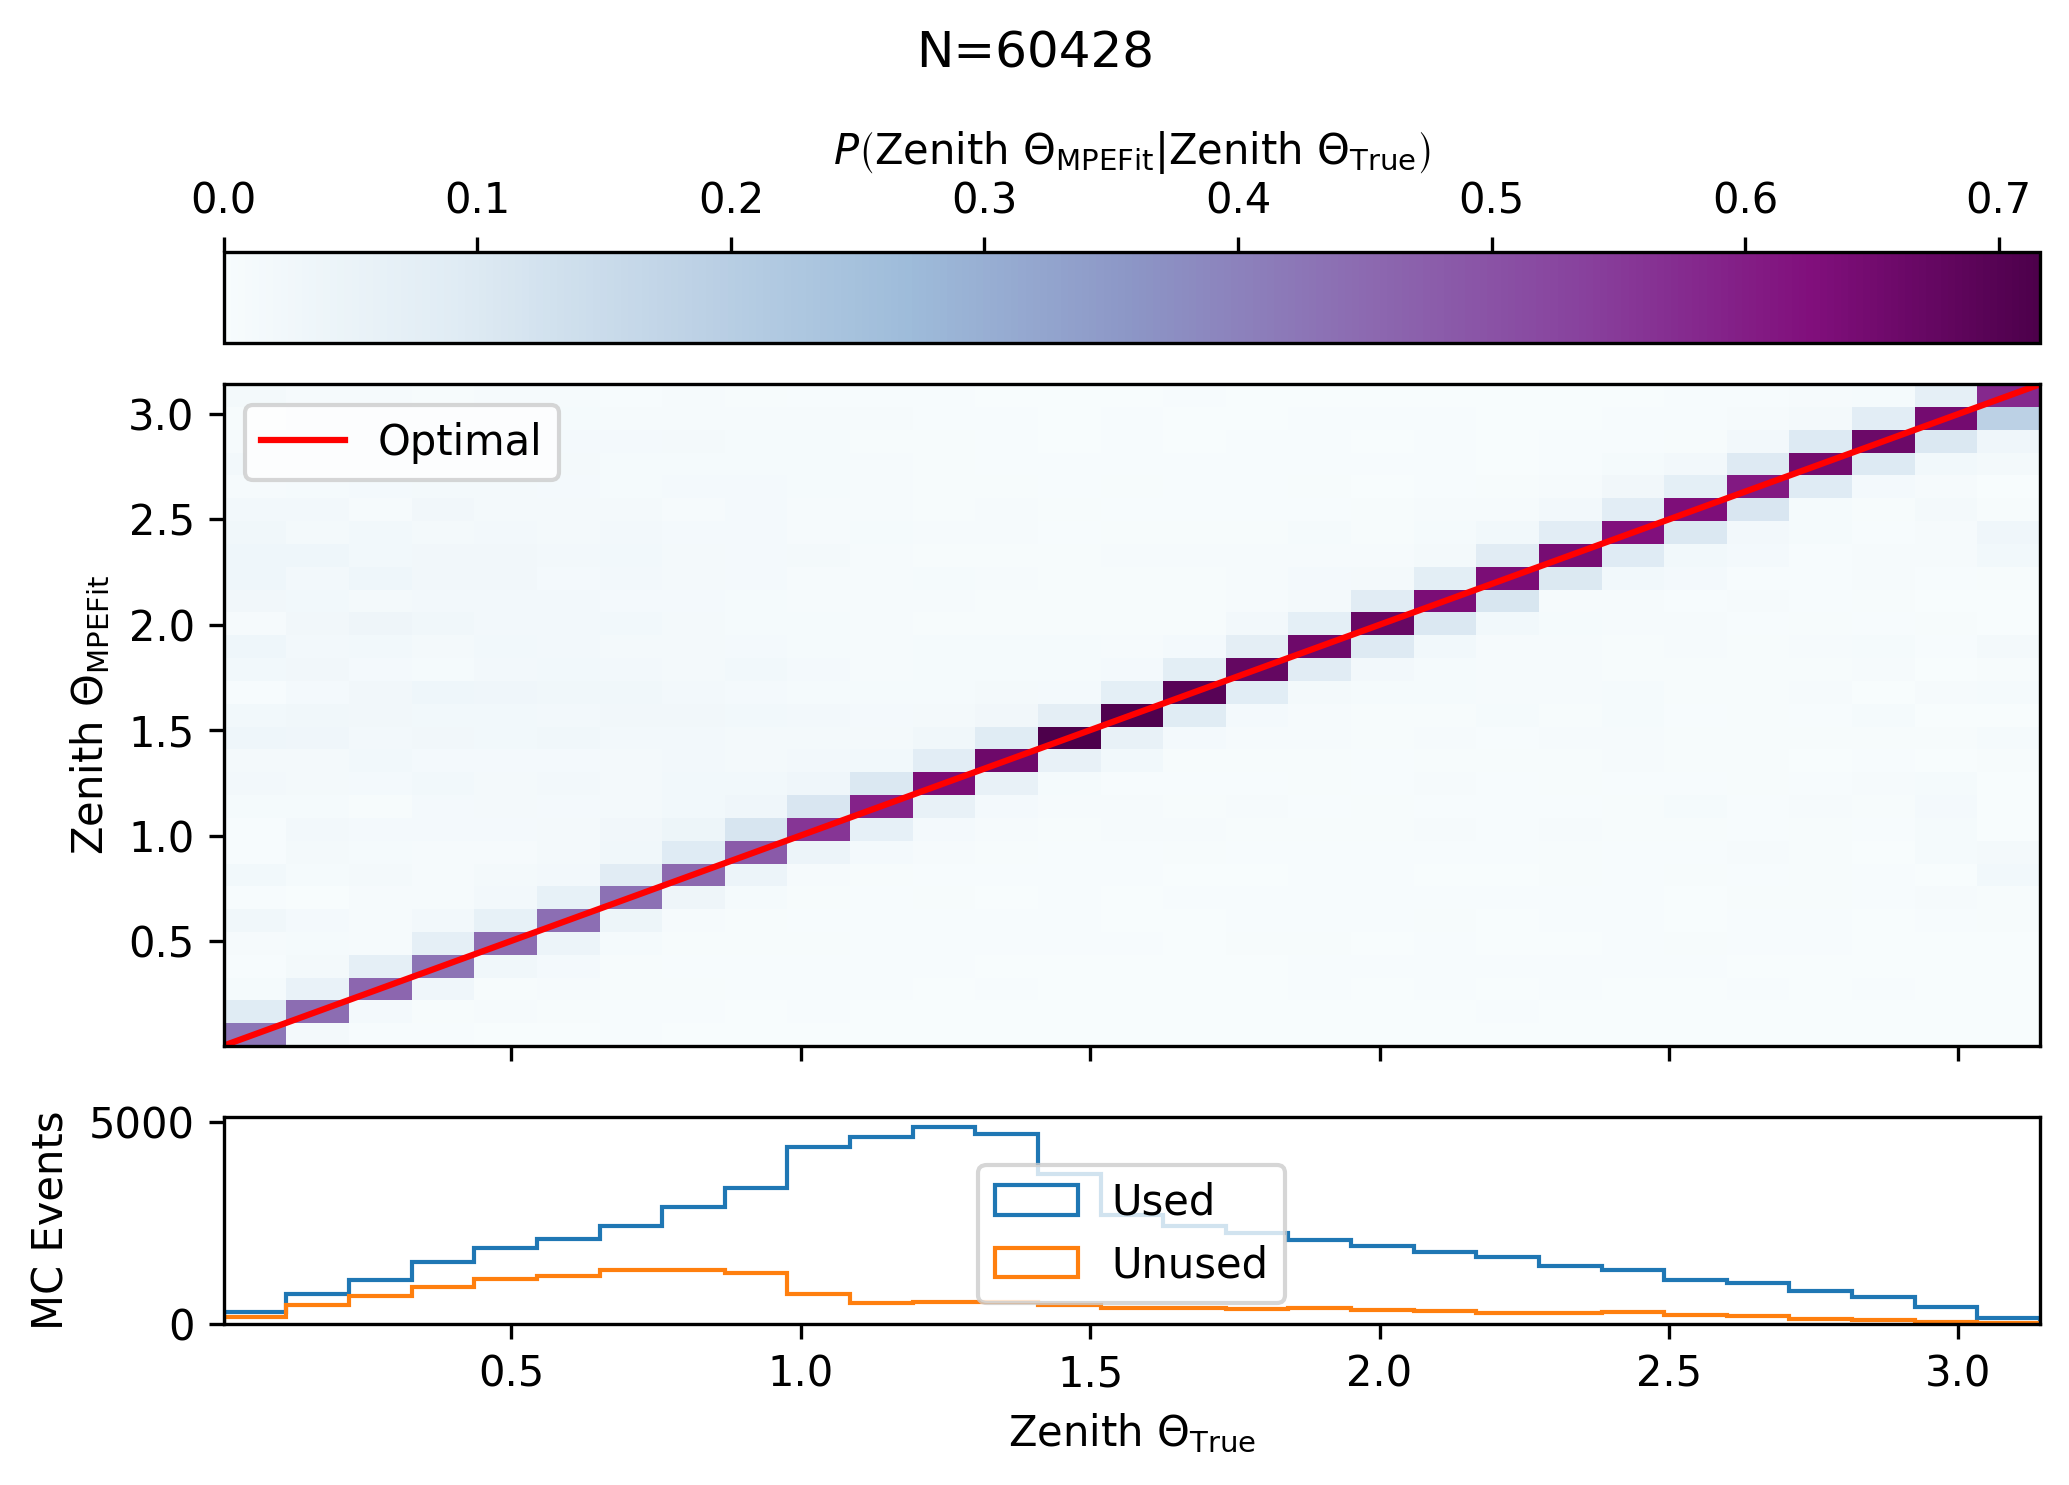
\includegraphics[width=.95\textwidth]{media/zenith_mpefit.png}
                    \caption*{\small Normalized zenith correlation for MPEFit}
                }
                \only<6>{
                    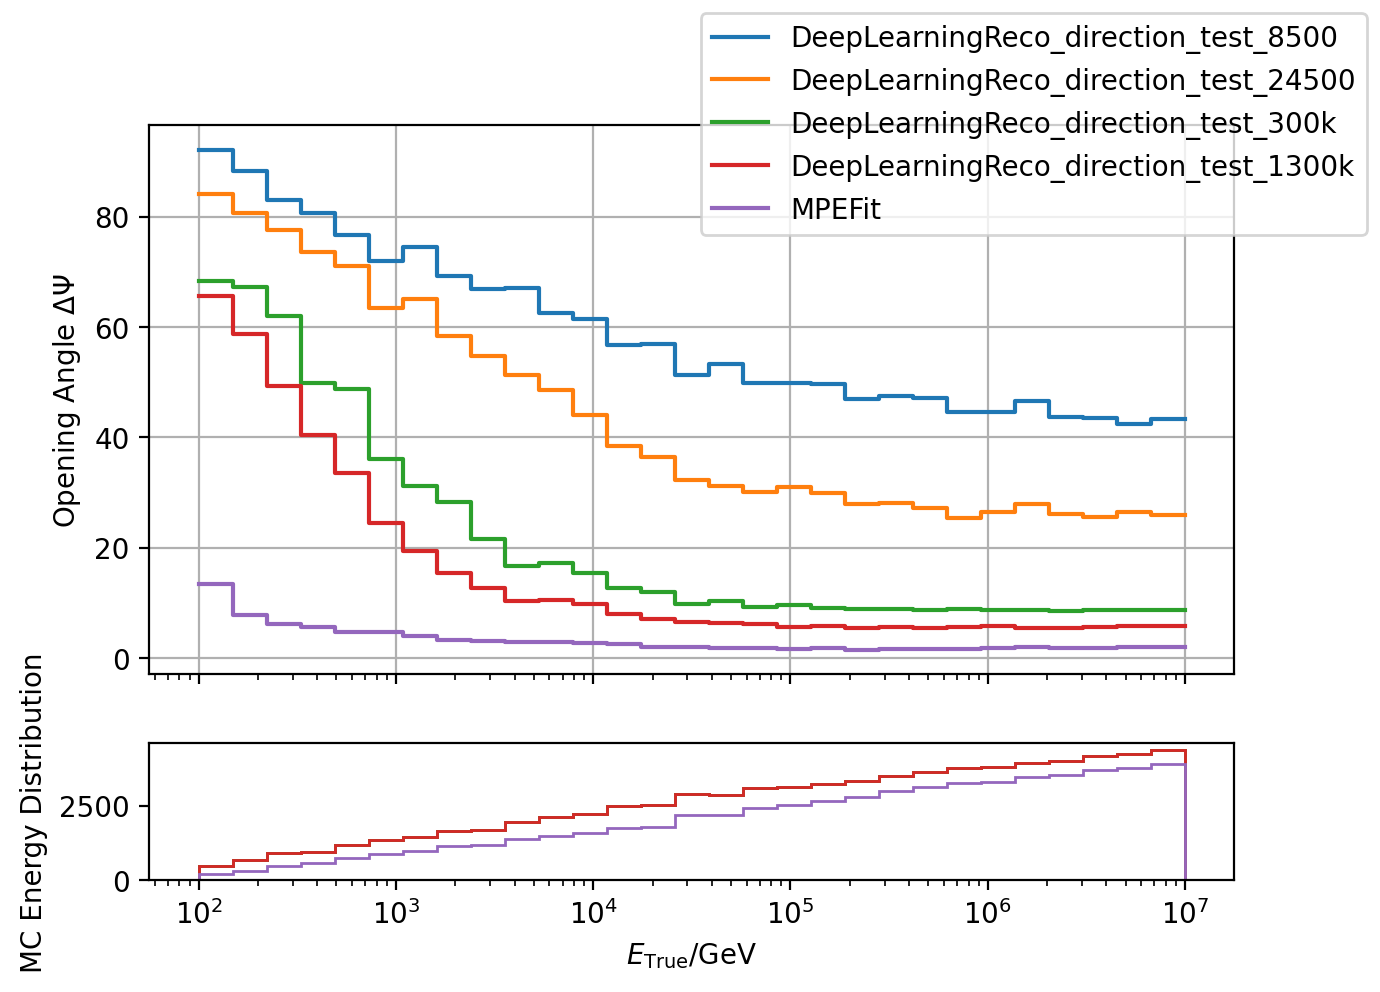
\includegraphics[width=.95\textwidth]{media/getting_started_opening_angle.png}
                    \caption*{\small Median opening angle vs. $E_\nu$}
                }
            \end{figure}
        \end{column}
    \end{columns}
\end{frame}
\begin{frame}{Generating Training Data}
    \begin{columns}
        \begin{column}{.35\textwidth}
            \begin{tabular}{>{\small\bf}r l}
                \toprule
                Features                  & 9         \\
                Training Dataset          & L2 11069  \\
                Batch Size                & 32        \\
                UDC conv. layers          & 4         \\
                LDC conv. layers          & 8         \\
                Hex. conv. layers         & 8         \\
                Dense layers              & 1\times50 \\
                $\rightarrow$ Free Params & 24532     \\
                \bottomrule
            \end{tabular}
        \end{column}
        \begin{column}{.65\textwidth}
            \begin{figure}
                \centering
                \only<1>{
                    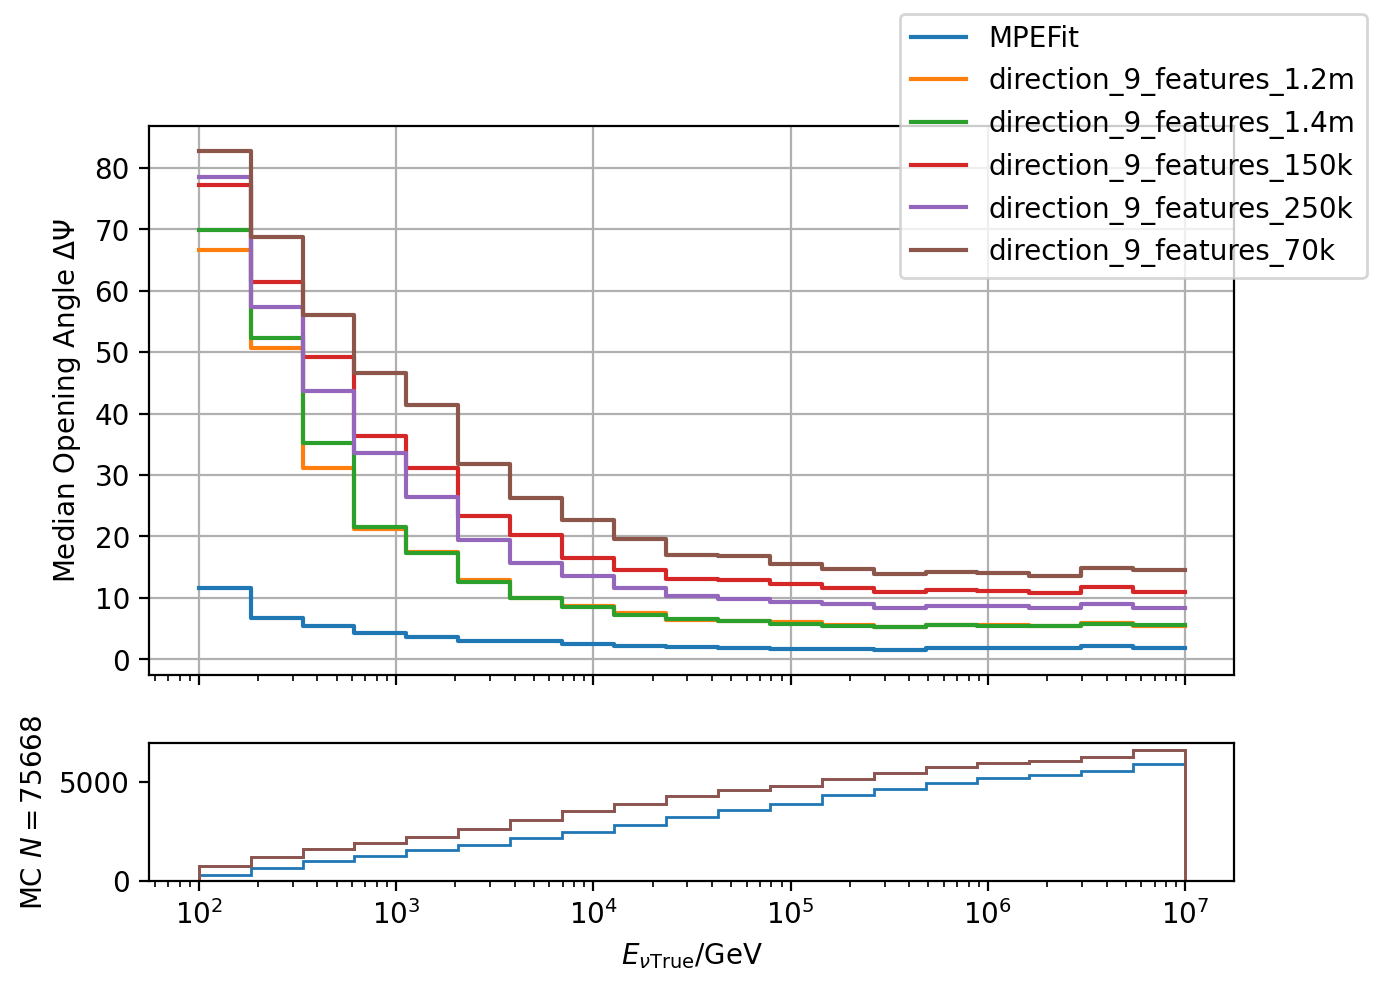
\includegraphics[width=.95\textwidth]{media/9_features_opening_angle.png}
                    \caption*{\small Median opening angle vs $E_\nu$}
                }
            \end{figure}
        \end{column}
    \end{columns}
\end{frame}
\begin{frame}{Improving the Model: Reduced Featureset}
    \begin{columns}
        \begin{column}{.35\textwidth}
            \begin{tabular}{>{\small\bf}r l}
                \toprule
                Features                  & 3         \\
                Training Dataset          & L2 11069  \\
                Batch Size                & 32        \\
                UDC conv. layers          & 4         \\
                LDC conv. layers          & 8         \\
                Hex. conv. layers         & 8         \\
                Dense layers              & 1\times50 \\
                $\rightarrow$ Free Params & 22462     \\
                \bottomrule
            \end{tabular}
        \end{column}
        \begin{column}{.65\textwidth}
            \only<1>{
                \begin{itemize}
                    \item 2070 parameters less
                    \item One test yielded 5-6 times faster training
                    \item Using
                          \begin{itemize}
                              \item total charge $c_{\mathrm{total}}$
                              \item first hit $t_{\mathrm{first}}$
                              \item charge weighted time std $t_{\mathrm{std}}$
                          \end{itemize}
                \end{itemize}
            }
            \only<2>{
                \begin{figure}
                    \centering
                    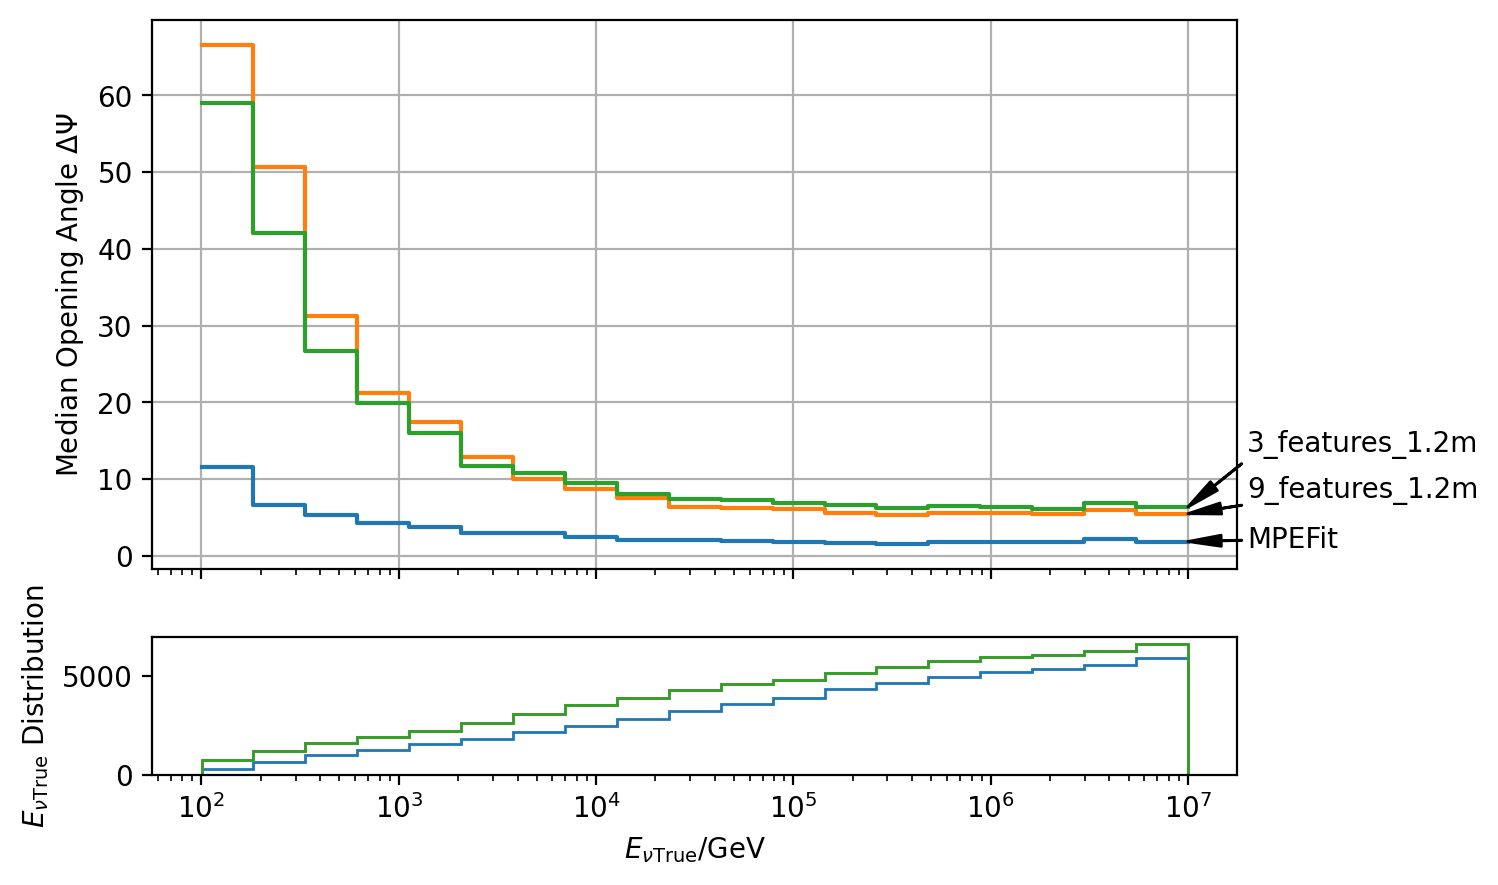
\includegraphics[width=.95\textwidth]{media/3_vs_9.png}
                    \caption*{\small Median opening angle vs $E_\nu$}
                \end{figure}}
        \end{column}
    \end{columns}
\end{frame}
\begin{frame}{Improving the Model: Higher Complexity}
    \begin{columns}
        \begin{column}{.35\textwidth}
            \begin{tabular}{>{\small\bf}r l}
                \toprule
                Features                  & 3          \\
                Training Dataset          & L2 11069   \\
                Batch Size                & 32         \\
                UDC conv. layers          & 4          \\
                LDC conv. layers          & 4          \\
                Hex. conv. layers         & 9          \\
                Dense layers              & 2\times100 \\
                $\rightarrow$ Free Params & 339467     \\
                \bottomrule
            \end{tabular}
        \end{column}
        \begin{column}{.65\textwidth}
            \only<1>{
                \begin{figure}
                    \centering
                    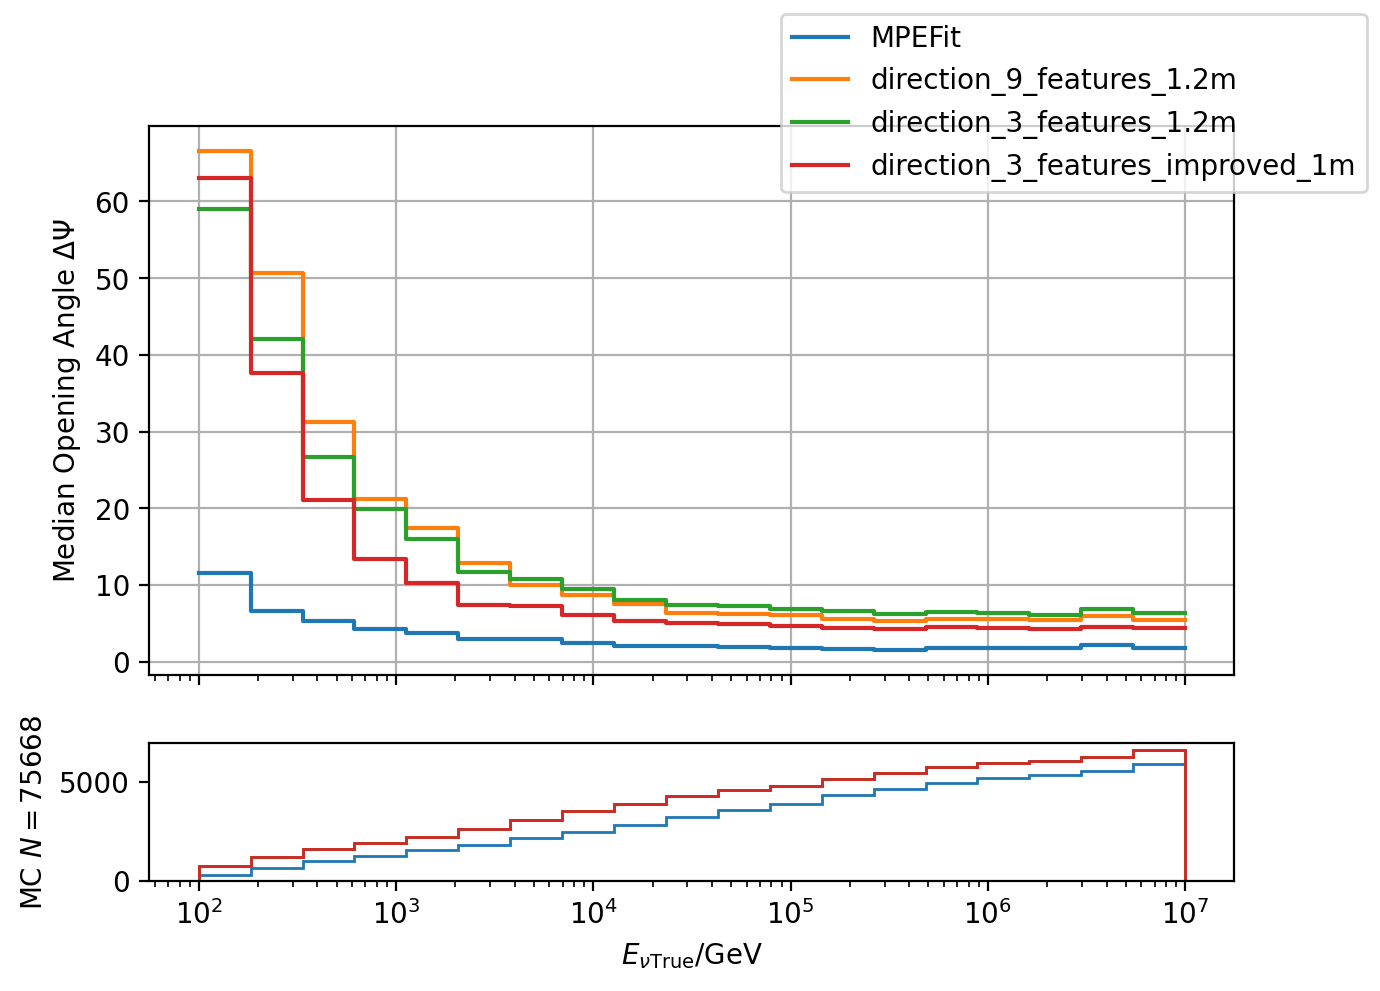
\includegraphics[width=.95\textwidth]{media/improved_model_compare.png}
                    \caption*{\small Median opening angle vs $E_\nu$}
                \end{figure}}
        \end{column}
    \end{columns}
\end{frame}
\begin{frame}{Improving the Model: Even Higher Complexity}
    \begin{columns}
        \begin{column}{.35\textwidth}
            \begin{tabular}{>{\small\bf}r l}
                \toprule
                Features                  & 3          \\
                Training Dataset          & L2 11069   \\
                Batch Size                & 32         \\
                UDC conv. layers          & 8          \\
                LDC conv. layers          & 14         \\
                Hex. conv. layers         & 20         \\
                Dense layers              & 2\times300 \\
                $\rightarrow$ Free Params & 5030912    \\
                \bottomrule
            \end{tabular}
        \end{column}
        \begin{column}{.65\textwidth}
            \only<1>{
                \begin{figure}
                    \centering
                    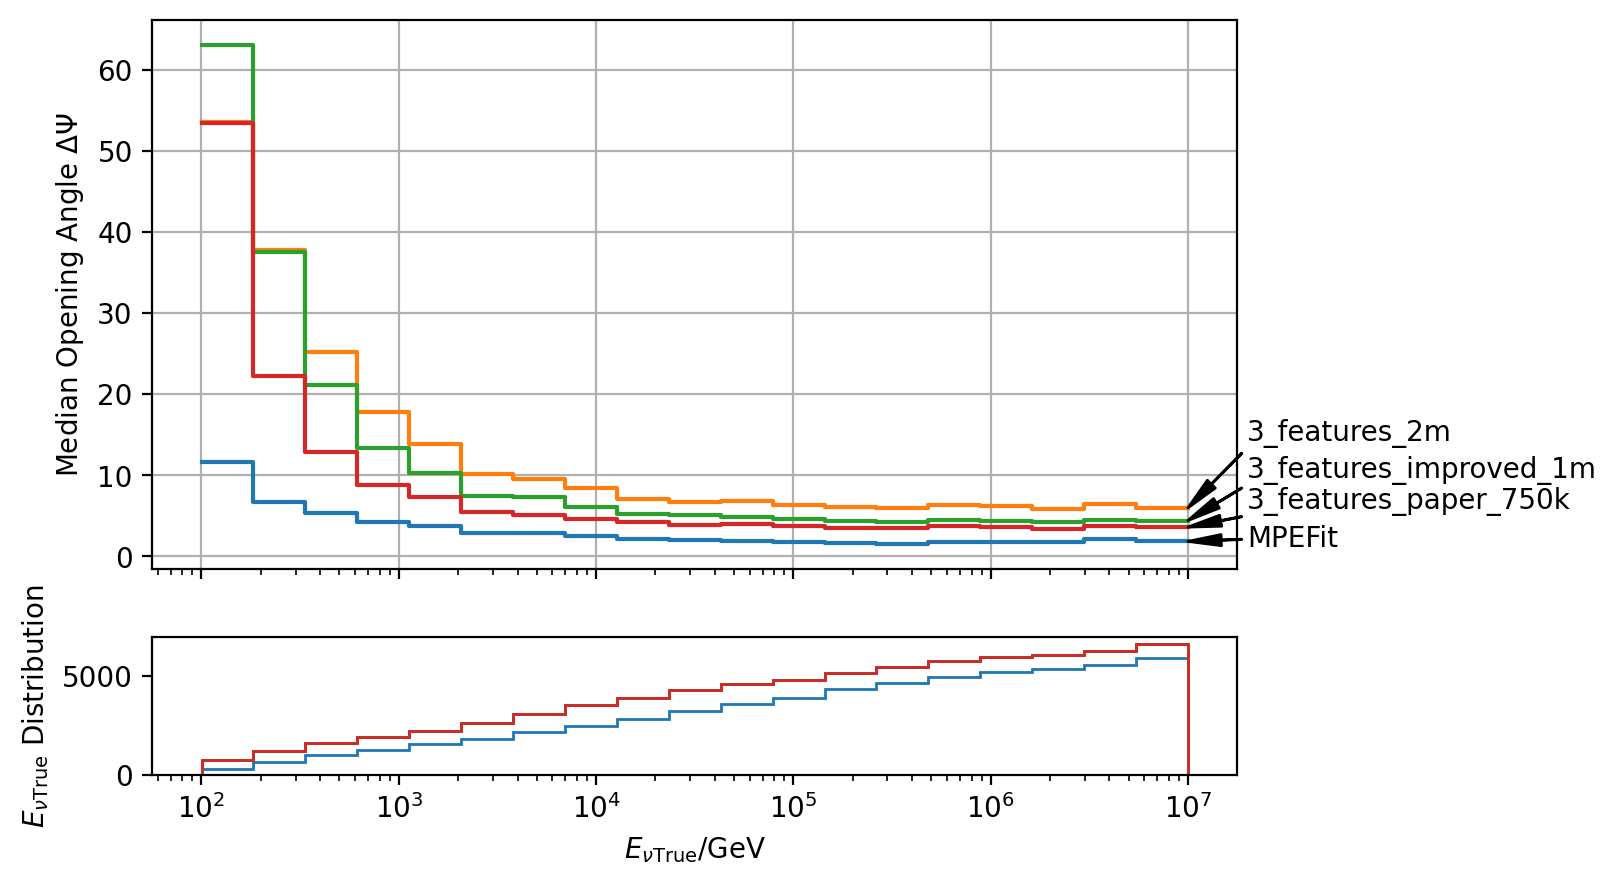
\includegraphics[width=.95\textwidth]{media/highest_complexity.png}
                    \caption*{\small Median opening angle vs $E_\nu$}
                \end{figure}}
        \end{column}
    \end{columns}
\end{frame}
\begin{frame}{Uncertainty Estimation with the High Complexity Model}
    \begin{figure}
        \centering
        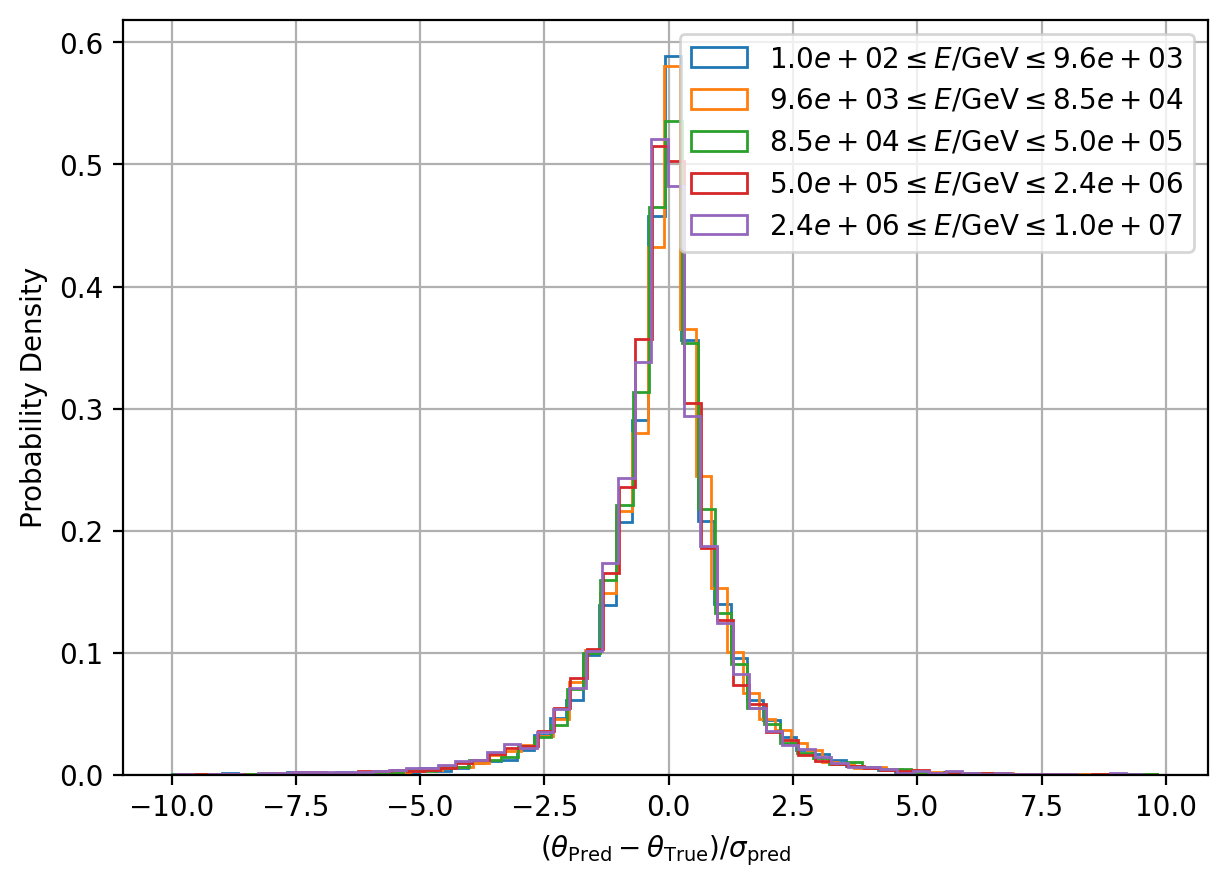
\includegraphics[width=.6\textwidth]{media/pulls.png}
        \caption*{\small Pull plot is peaked compared to expected Gaussian shape, but stable in $E_\nu$}
    \end{figure}
\end{frame}
\begin{frame}{Uncertainty Estimation with the High Complexity Model}
    \begin{figure}
        \centering
        \only<1>{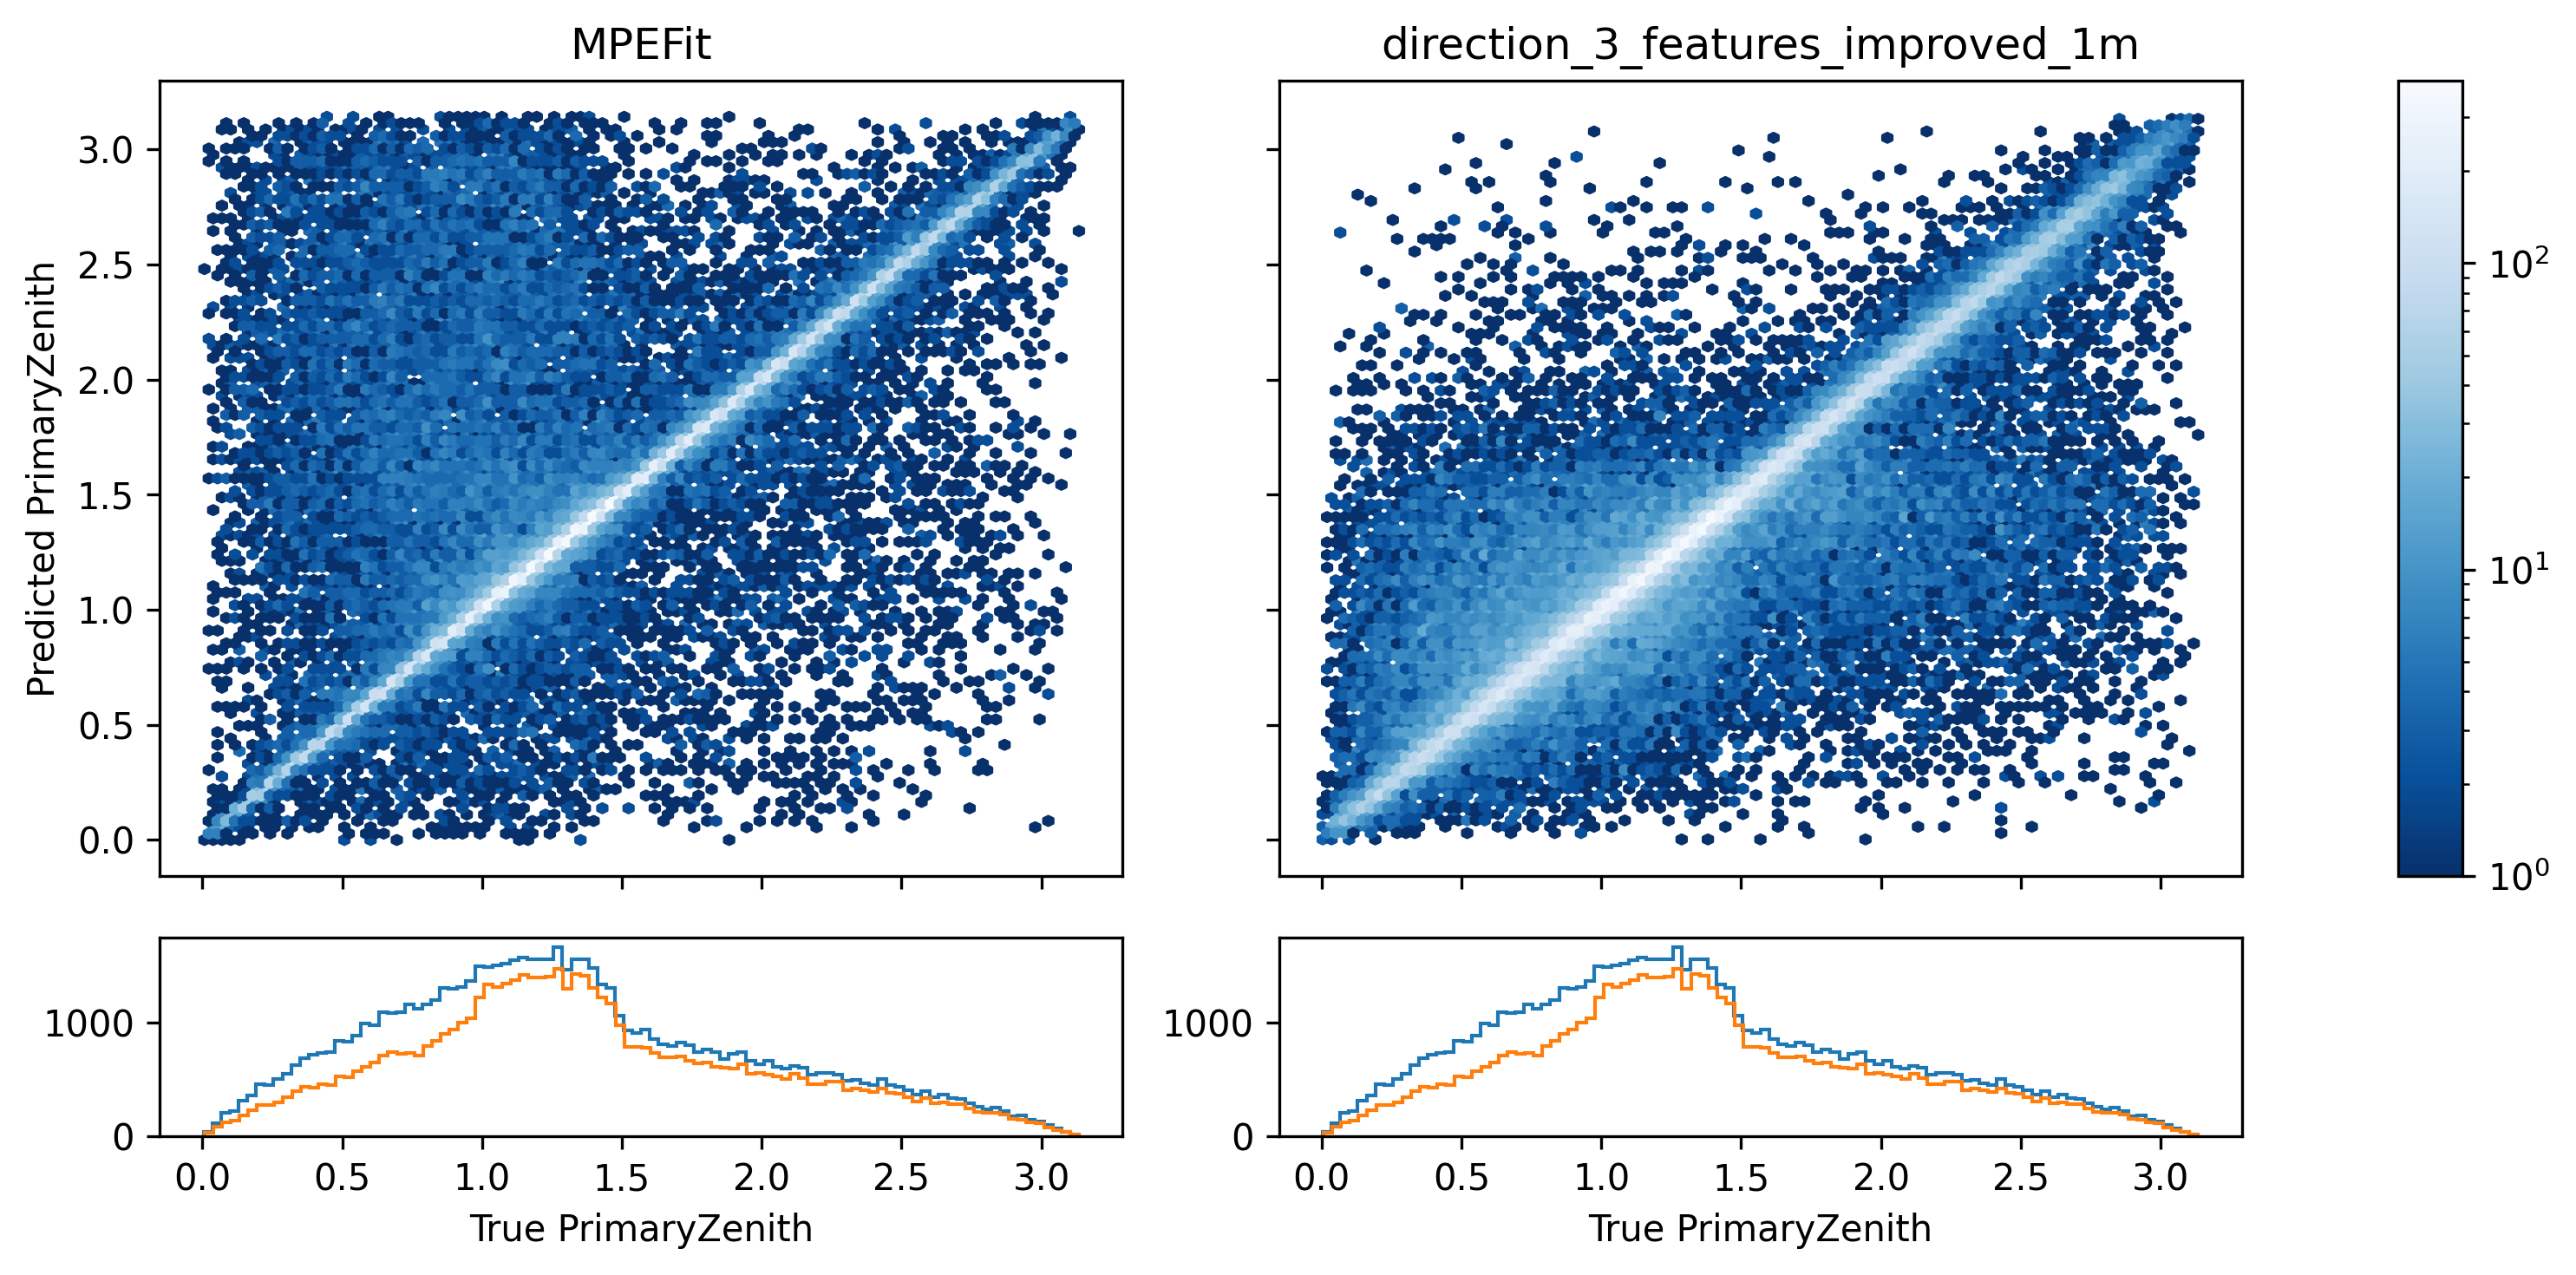
\includegraphics[width=.8\textwidth]{media/scatter_uncertainty.png}}
        \only<2>{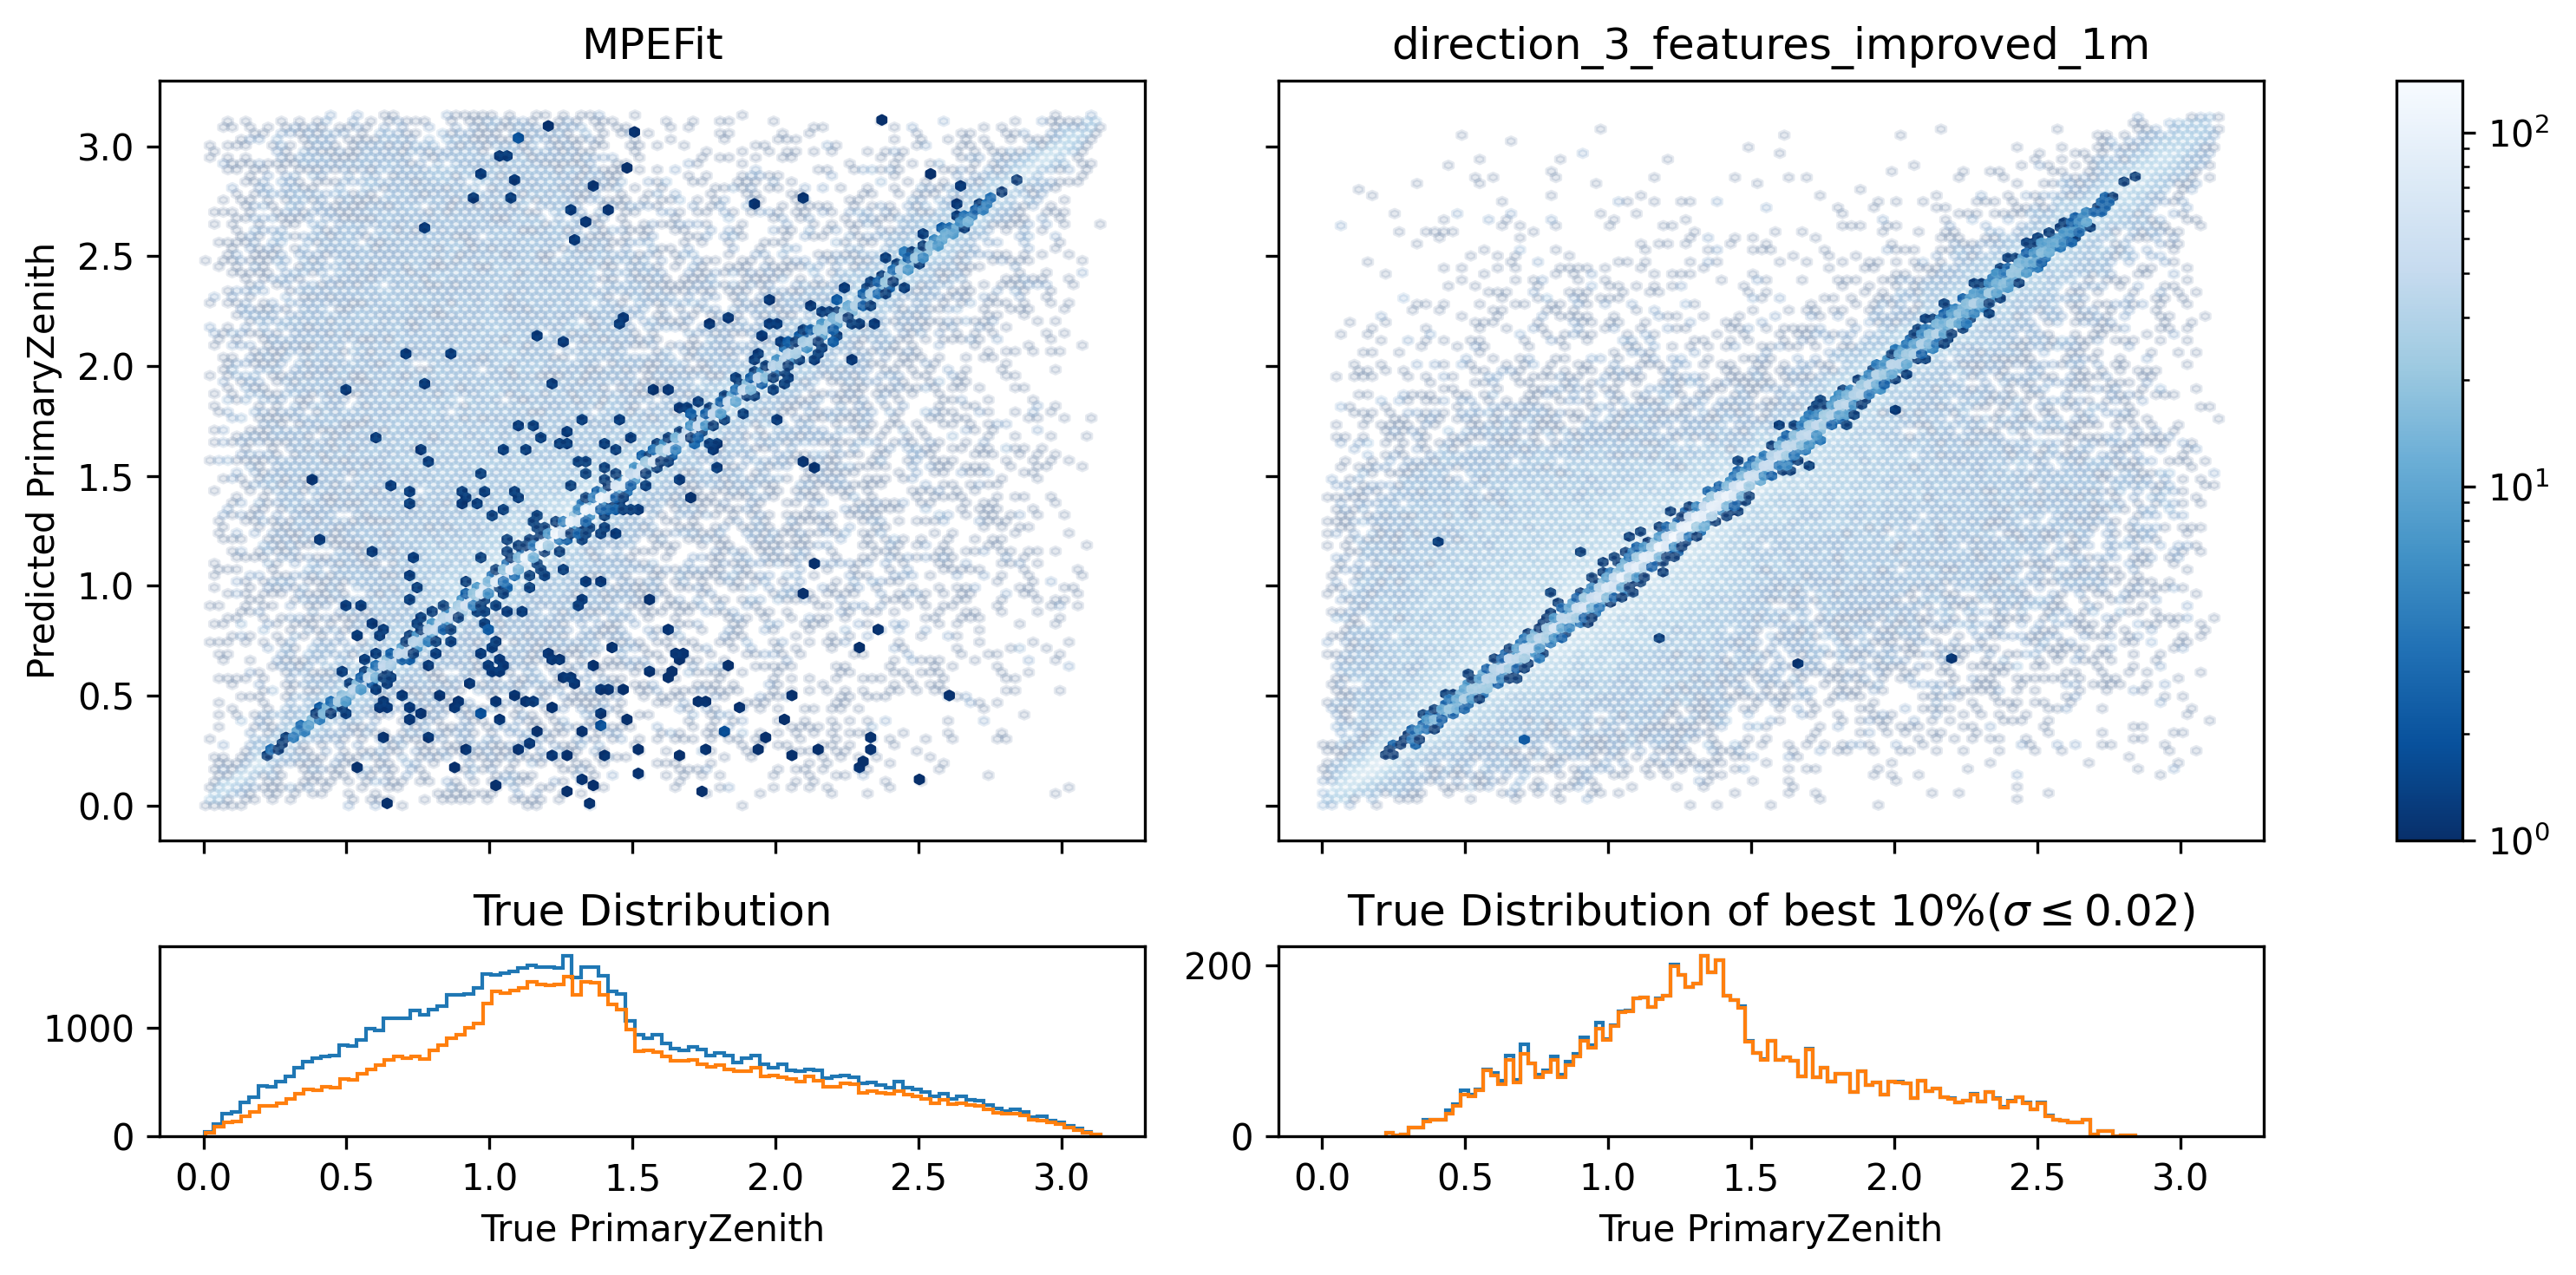
\includegraphics[width=.8\textwidth]{media/scatter_uncertainty_best.png}}
        \only<1>{\caption*{\small Hexagonal 2D-Bin plot in logarithmic color scale}}
        \only<2>{\caption*{\small Only showing 10\% of events with the lowest uncertainty estimate from DNN}}
    \end{figure}
\end{frame}
\begin{frame}{What's next?}
    \begin{itemize}
        \item Getting the software to run on the local SU cluster using (singularity) containers
              \footnote{We already have docker images available: \tiny\url{https://hub.docker.com/repository/docker/theludwig/dnn_reco}}
        \item More complex models, less training
        \item Training with opening angle loss-function
        \item Understanding distribution of uncertainty prediction and pulls
        \item Start with MSE Loss-Function and move later to Gaussian Likelihood
        \item Finish by \emph{only} training uncertainty subnetwork
    \end{itemize}
\end{frame}
\begin{frame}

    \section*{Questions?}

\end{frame}

\begin{frame}
  \nocite{*}
  \printbibliography
\end{frame}

\end{document}

